\documentclass{book}
\usepackage[utf8]{inputenc}
\usepackage[top=1in]{geometry}
\usepackage{graphicx}
\usepackage{booktabs}
\usepackage{amsmath}
\usepackage{amsthm}
\usepackage[only]{excludeonly}
\usepackage{tikz}
\usepackage{verbatim}
\usetikzlibrary{circuits.logic.US,positioning,calc} 
\usepackage[american]{circuitikz}
\usepackage{enumitem,amssymb}
\usepackage{url}
\usepackage{wrapfig}
\usepackage{easy-todo}

% \newlist{todolist}{itemize}{2}
% \setlist[todolist]{label=$\square$}
% \usepackage{pifont}
% \newcommand{\cmark}{\ding{51}}%
% \newcommand{\xmark}{\ding{55}}%
% \newcommand{\done}{\rlap{$\square$}{\raisebox{2pt}{\large\hspace{1pt}\cmark}}%
%   \hspace{-2.5pt}}
% \newcommand{\wontfix}{\rlap{$\square$}{\large\hspace{1pt}\xmark}}

% https://tex.stackexchange.com/questions/140567/drawing-karnaughs-maps-in-latex
\usepackage{tikz}
\usetikzlibrary{matrix,calc}

%isolated term
%#1 - Optional. Space between node and grouping line. Default=0
%#2 - node
%#3 - filling color
\newcommand{\implicantsol}[3][0]{
    \draw[rounded corners=3pt, fill=#3, opacity=0.3] ($(#2.north west)+(135:#1)$) rectangle ($(#2.south east)+(-45:#1)$);
    }


%internal group
%#1 - Optional. Space between node and grouping line. Default=0
%#2 - top left node
%#3 - bottom right node
%#4 - filling color
\newcommand{\implicant}[4][0]{
    \draw[rounded corners=3pt, fill=#4, opacity=0.3] ($(#2.north west)+(135:#1)$) rectangle ($(#3.south east)+(-45:#1)$);
    }

%group lateral borders
%#1 - Optional. Space between node and grouping line. Default=0
%#2 - top left node
%#3 - bottom right node
%#4 - filling color
\newcommand{\implicantcostats}[4][0]{
    \draw[rounded corners=3pt, fill=#4, opacity=0.3] ($(rf.east |- #2.north)+(90:#1)$)-| ($(#2.east)+(0:#1)$) |- ($(rf.east |- #3.south)+(-90:#1)$);
    \draw[rounded corners=3pt, fill=#4, opacity=0.3] ($(cf.west |- #2.north)+(90:#1)$) -| ($(#3.west)+(180:#1)$) |- ($(cf.west |- #3.south)+(-90:#1)$);
}

%group top-bottom borders
%#1 - Optional. Space between node and grouping line. Default=0
%#2 - top left node
%#3 - bottom right node
%#4 - filling color
\newcommand{\implicantdaltbaix}[4][0]{
    \draw[rounded corners=3pt, fill=#4, opacity=0.3] ($(cf.south -| #2.west)+(180:#1)$) |- ($(#2.south)+(-90:#1)$) -| ($(cf.south -| #3.east)+(0:#1)$);
    \draw[rounded corners=3pt, fill=#4, opacity=0.3] ($(rf.north -| #2.west)+(180:#1)$) |- ($(#3.north)+(90:#1)$) -| ($(rf.north -| #3.east)+(0:#1)$);
}

%group corners
%#1 - Optional. Space between node and grouping line. Default=0
%#2 - filling color
\newcommand{\implicantcantons}[2][0]{
    \draw[rounded corners=3pt, opacity=.3] ($(rf.east |- 0.south)+(-90:#1)$) -| ($(0.east |- cf.south)+(0:#1)$);
    \draw[rounded corners=3pt, opacity=.3] ($(rf.east |- 8.north)+(90:#1)$) -| ($(8.east |- rf.north)+(0:#1)$);
    \draw[rounded corners=3pt, opacity=.3] ($(cf.west |- 2.south)+(-90:#1)$) -| ($(2.west |- cf.south)+(180:#1)$);
    \draw[rounded corners=3pt, opacity=.3] ($(cf.west |- 10.north)+(90:#1)$) -| ($(10.west |- rf.north)+(180:#1)$);
    \fill[rounded corners=3pt, fill=#2, opacity=.3] ($(rf.east |- 0.south)+(-90:#1)$) -|  ($(0.east |- cf.south)+(0:#1)$) [sharp corners] ($(rf.east |- 0.south)+(-90:#1)$) |-  ($(0.east |- cf.south)+(0:#1)$) ;
    \fill[rounded corners=3pt, fill=#2, opacity=.3] ($(rf.east |- 8.north)+(90:#1)$) -| ($(8.east |- rf.north)+(0:#1)$) [sharp corners] ($(rf.east |- 8.north)+(90:#1)$) |- ($(8.east |- rf.north)+(0:#1)$) ;
    \fill[rounded corners=3pt, fill=#2, opacity=.3] ($(cf.west |- 2.south)+(-90:#1)$) -| ($(2.west |- cf.south)+(180:#1)$) [sharp corners]($(cf.west |- 2.south)+(-90:#1)$) |- ($(2.west |- cf.south)+(180:#1)$) ;
    \fill[rounded corners=3pt, fill=#2, opacity=.3] ($(cf.west |- 10.north)+(90:#1)$) -| ($(10.west |- rf.north)+(180:#1)$) [sharp corners] ($(cf.west |- 10.north)+(90:#1)$) |- ($(10.west |- rf.north)+(180:#1)$) ;
}

%Empty Karnaugh map 4x4
\newenvironment{Karnaugh}[2]%
{
\begin{tikzpicture}[baseline=(current bounding box.north),scale=0.8]
\draw (0,0) grid (4,4);
\draw (0,4) -- node [pos=0.7,above right,anchor=south west] {#1} node [pos=0.7,below left,anchor=north east] {#2} ++(135:1);
%
\matrix (mapa) [matrix of nodes,
        column sep={0.8cm,between origins},
        row sep={0.8cm,between origins},
        every node/.style={minimum size=0.3mm},
        anchor=2.center,
        ampersand replacement=\&] at (0.5,0.5)
{
                       \& |(c00)| 00         \& |(c01)| 01         \& |(c11)| 11         \& |(c10)| 10         \& |(cf)| \phantom{00} \\
|(r00)| 00             \& |(0)|  \phantom{0} \& |(4)|  \phantom{0} \& |(12)|  \phantom{0} \& |(8)|  \phantom{0} \&                     \\
|(r01)| 01             \& |(1)|  \phantom{0} \& |(5)|  \phantom{0} \& |(13)|  \phantom{0} \& |(9)|  \phantom{0} \&                     \\
|(r11)| 11             \& |(3)| \phantom{0} \& |(7)| \phantom{0} \& |(15)| \phantom{0} \& |(11)| \phantom{0} \&                     \\
|(r10)| 10             \& |(2)|  \phantom{0} \& |(6)|  \phantom{0} \& |(14)| \phantom{0} \& |(10)| \phantom{0} \&                     \\
|(rf) | \phantom{00}   \&                    \&                    \&                    \&                    \&                     \\
};
}%
{
\end{tikzpicture}
}

%Empty Karnaugh map 2x4
\newenvironment{Karnaughvuit}%
{
\begin{tikzpicture}[baseline=(current bounding box.north),scale=0.8]
\draw (0,0) grid (4,2);
\draw (0,2) -- node [pos=0.7,above right,anchor=south west] {AB} node [pos=0.7,below left,anchor=north east] {C} ++(135:1);
%
\matrix (mapa) [matrix of nodes,
        column sep={0.8cm,between origins},
        row sep={0.8cm,between origins},
        every node/.style={minimum size=0.3mm},
        anchor=1.center,
        ampersand replacement=\&] at (0.5,0.5)
{
                      \& |(c00)| 00         \& |(c01)| 01         \& |(c11)| 11         \& |(c10)| 10         \& |(cf)| \phantom{00} \\
|(r00)| 0             \& |(0)|  \phantom{0} \& |(2)|  \phantom{0} \& |(6)|  \phantom{0} \& |(4)|  \phantom{0} \&                     \\
|(r01)| 1             \& |(1)|  \phantom{0} \& |(3)|  \phantom{0} \& |(7)|  \phantom{0} \& |(5)|  \phantom{0} \&                     \\
|(rf) | \phantom{00}  \&                    \&                    \&                    \&                    \&                     \\
};
}%
{
\end{tikzpicture}
}

%Empty Karnaugh map 2x2
\newenvironment{Karnaughquatre}%
{
\begin{tikzpicture}[baseline=(current bounding box.north),scale=0.8]
\draw (0,0) grid (2,2);
\draw (0,2) -- node [pos=0.7,above right,anchor=south west] {A} node [pos=0.7,below left,anchor=north east] {B} ++(135:1);
%
\matrix (mapa) [matrix of nodes,
        column sep={0.8cm,between origins},
        row sep={0.8cm,between origins},
        every node/.style={minimum size=0.3mm},
        anchor=1.center,
        ampersand replacement=\&] at (0.5,0.5)
{
          \& |(c00)| 0          \& |(c01)| 1  \\
|(r00)| 0 \& |(0)|  \phantom{0} \& |(2)|  \phantom{0} \\
|(r01)| 1 \& |(1)|  \phantom{0} \& |(3)|  \phantom{0} \\
};
}%
{
\end{tikzpicture}
}

%Defines 8 or 16 values (0,1,X)
\newcommand{\contingut}[1]{%
\foreach \x [count=\xi from 0]  in {#1}
     \path (\xi) node {\x};
}

%Places 1 in listed positions
\newcommand{\minterms}[1]{%
    \foreach \x in {#1}
        \path (\x) node {1};
}

%Places 0 in listed positions
\newcommand{\maxterms}[1]{%
    \foreach \x in {#1}
        \path (\x) node {0};
}

%Places X in listed positions
\newcommand{\indeterminats}[1]{%
    \foreach \x in {#1}
        \path (\x) node {X};
}

% Places m_{x} in listed positions
\newcommand{\phminterms}[1]{%
  \foreach \x in {#1}
  \path (\x) node {$m_{\x}$};
}

% Places m_{16+x} in listed positions
\newcommand{\phmintermssixt}[1]{%
  \foreach [evaluate={\y=int(16+\x)}] \x in {#1}
  \path (\x) node {$m_{\y}$};
}

% Calligraphic fonts
\newcommand{\calA}{{\cal A}}
\newcommand{\calB}{{\cal B}}
\newcommand{\calC}{{\cal C}}
\newcommand{\calD}{{\cal D}}
\newcommand{\calE}{{\cal E}}
\newcommand{\calF}{{\cal F}}
\newcommand{\calG}{{\cal G}}
\newcommand{\calH}{{\cal H}}
\newcommand{\calI}{{\cal I}}
\newcommand{\calJ}{{\cal J}}
\newcommand{\calK}{{\cal K}}
\newcommand{\calL}{{\cal L}}
\newcommand{\calM}{{\cal M}}
\newcommand{\calN}{{\cal N}}
\newcommand{\calO}{{\cal O}}
\newcommand{\calP}{{\cal P}}
\newcommand{\calQ}{{\cal Q}}
\newcommand{\calR}{{\cal R}}
\newcommand{\calS}{{\cal S}}
\newcommand{\calT}{{\cal T}}
\newcommand{\calU}{{\cal U}}
\newcommand{\calV}{{\cal V}}
\newcommand{\calW}{{\cal W}}
\newcommand{\calX}{{\cal X}}
\newcommand{\calY}{{\cal Y}}
\newcommand{\calZ}{{\cal Z}}

% Sets:
\newcommand{\setA}{\textsf{A}}
\newcommand{\setB}{\textsf{B}}
\newcommand{\setC}{\textsf{C}}
\newcommand{\setD}{\textsf{D}}
\newcommand{\setE}{\textsf{E}}
\newcommand{\setF}{\textsf{F}}
\newcommand{\setG}{\textsf{G}}
\newcommand{\setH}{\textsf{H}}
\newcommand{\setI}{\textsf{I}}
\newcommand{\setJ}{\textsf{J}}
\newcommand{\setK}{\textsf{K}}
\newcommand{\setL}{\textsf{L}}
\newcommand{\setM}{\textsf{M}}
\newcommand{\setN}{\textsf{N}}
\newcommand{\setO}{\textsf{O}}
\newcommand{\setP}{\textsf{P}}
\newcommand{\setQ}{\textsf{Q}}
\newcommand{\setR}{\textsf{R}}
\newcommand{\setS}{\textsf{S}}
\newcommand{\setT}{\textsf{T}}
\newcommand{\setU}{\textsf{U}}
\newcommand{\setV}{\textsf{V}}
\newcommand{\setW}{\textsf{W}}
\newcommand{\setX}{\textsf{X}}
\newcommand{\setY}{\textsf{Y}}
\newcommand{\setZ}{\textsf{Z}}

% Vectors
\newcommand{\bfa}{\mathbf{a}}
\newcommand{\bfb}{\mathbf{b}}
\newcommand{\bfc}{\mathbf{c}}
\newcommand{\bfd}{\mathbf{d}}
\newcommand{\bfe}{\mathbf{e}}
\newcommand{\bff}{\mathbf{f}}
\newcommand{\bfg}{\mathbf{g}}
\newcommand{\bfh}{\mathbf{h}}
\newcommand{\bfi}{\mathbf{i}}
\newcommand{\bfj}{\mathbf{j}}
\newcommand{\bfk}{\mathbf{k}}
\newcommand{\bfl}{\mathbf{l}}
\newcommand{\bfm}{\mathbf{m}}
\newcommand{\bfn}{\mathbf{n}}
\newcommand{\bfo}{\mathbf{o}}
\newcommand{\bfp}{\mathbf{p}}
\newcommand{\bfq}{\mathbf{q}}
\newcommand{\bfr}{\mathbf{r}}
\newcommand{\bfs}{\mathbf{s}}
\newcommand{\bft}{\mathbf{t}}
\newcommand{\bfu}{\mathbf{u}}
\newcommand{\bfv}{\mathbf{v}}
\newcommand{\bfw}{\mathbf{w}}
\newcommand{\bfx}{\mathbf{x}}
\newcommand{\bfy}{\mathbf{y}}
\newcommand{\bfz}{\mathbf{z}}


\newcommand{\bfalpha}{\boldsymbol{\alpha}}
\newcommand{\bfbeta}{\boldsymbol{\beta}}
\newcommand{\bfgamma}{\boldsymbol{\gamma}}
\newcommand{\bfdelta}{\boldsymbol{\delta}}
\newcommand{\bfepsilon}{\boldsymbol{\epsilon}}
\newcommand{\bfzeta}{\boldsymbol{\zeta}}
\newcommand{\bfeta}{\boldsymbol{\eta}}
\newcommand{\bftheta}{\boldsymbol{\theta}}
\newcommand{\bfiota}{\boldsymbol{\iota}}
\newcommand{\bfkappa}{\boldsymbol{\kappa}}
\newcommand{\bflambda}{\boldsymbol{\lambda}}
\newcommand{\bfmu}{\boldsymbol{\mu}}
\newcommand{\bfnu}{\boldsymbol{\nu}}
\newcommand{\bfomicron}{\boldsymbol{\omicron}}
\newcommand{\bfpi}{\boldsymbol{\pi}}
\newcommand{\bfrho}{\boldsymbol{\rho}}
\newcommand{\bfsigma}{\boldsymbol{\sigma}}
\newcommand{\bftau}{\boldsymbol{\tau}}
\newcommand{\bfupsilon}{\boldsymbol{\upsilon}}
\newcommand{\bfphi}{\boldsymbol{\phi}}
\newcommand{\bfchi}{\boldsymbol{\chi}}
\newcommand{\bfpsi}{\boldsymbol{\psi}}
\newcommand{\bfomega}{\boldsymbol{\omega}}
\newcommand{\bfxi}{\boldsymbol{\xi}}
\newcommand{\bfell}{\boldsymbol{\ell}}

% Matrices
\newcommand{\bfA}{\mathbf{A}}
\newcommand{\bfB}{\mathbf{B}}
\newcommand{\bfC}{\mathbf{C}}
\newcommand{\bfD}{\mathbf{D}}
\newcommand{\bfE}{\mathbf{E}}
\newcommand{\bfF}{\mathbf{F}}
\newcommand{\bfG}{\mathbf{G}}
\newcommand{\bfH}{\mathbf{H}}
\newcommand{\bfI}{\mathbf{I}}
\newcommand{\bfJ}{\mathbf{J}}
\newcommand{\bfK}{\mathbf{K}}
\newcommand{\bfL}{\mathbf{L}}
\newcommand{\bfM}{\mathbf{M}}
\newcommand{\bfN}{\mathbf{N}}
\newcommand{\bfO}{\mathbf{O}}
\newcommand{\bfP}{\mathbf{P}}
\newcommand{\bfQ}{\mathbf{Q}}
\newcommand{\bfR}{\mathbf{R}}
\newcommand{\bfS}{\mathbf{S}}
\newcommand{\bfT}{\mathbf{T}}
\newcommand{\bfU}{\mathbf{U}}
\newcommand{\bfV}{\mathbf{V}}
\newcommand{\bfW}{\mathbf{W}}
\newcommand{\bfX}{\mathbf{X}}
\newcommand{\bfY}{\mathbf{Y}}
\newcommand{\bfZ}{\mathbf{Z}}


\newcommand{\bfGamma}{\boldsymbol{\Gamma}}
\newcommand{\bfDelta}{\boldsymbol{\Delta}}
\newcommand{\bfTheta}{\boldsymbol{\Theta}}
\newcommand{\bfLambda}{\boldsymbol{\Lambda}}
\newcommand{\bfPi}{\boldsymbol{\Pi}}
\newcommand{\bfSigma}{\boldsymbol{\Sigma}}
\newcommand{\bfUpsilon}{\boldsymbol{\Upsilon}}
\newcommand{\bfPhi}{\boldsymbol{\Phi}}
\newcommand{\bfPsi}{\boldsymbol{\Psi}}
\newcommand{\bfOmega}{\boldsymbol{\Omega}}


% Blackboard Bold:
\newcommand{\bbA}{\mathbb{A}}
\newcommand{\bbB}{\mathbb{B}}
\newcommand{\bbC}{\mathbb{C}}
\newcommand{\bbD}{\mathbb{D}}
\newcommand{\bbE}{\mathbb{E}}
\newcommand{\bbF}{\mathbb{F}}
\newcommand{\bbG}{\mathbb{G}}
\newcommand{\bbH}{\mathbb{H}}
\newcommand{\bbI}{\mathbb{I}}
\newcommand{\bbJ}{\mathbb{J}}
\newcommand{\bbK}{\mathbb{K}}
\newcommand{\bbL}{\mathbb{L}}
\newcommand{\bbM}{\mathbb{M}}
\newcommand{\bbN}{\mathbb{N}}
\newcommand{\bbO}{\mathbb{O}}
\newcommand{\bbP}{\mathbb{P}}
\newcommand{\bbQ}{\mathbb{Q}}
\newcommand{\bbR}{\mathbb{R}}
\newcommand{\bbS}{\mathbb{S}}
\newcommand{\bbT}{\mathbb{T}}
\newcommand{\bbU}{\mathbb{U}}
\newcommand{\bbV}{\mathbb{V}}
\newcommand{\bbW}{\mathbb{W}}
\newcommand{\bbX}{\mathbb{X}}
\newcommand{\bbY}{\mathbb{Y}}
\newcommand{\bbZ}{\mathbb{Z}}




\graphicspath{{0831-number-system/}
{0831-number-system}
{0907-boolean-algebra}
{0916-K-maps}
{0928-adders-carry-ahead}
{0928-quine-mccluskey}
{0930-review}
{1014-analog-details}
{1024-cmos-gate-review}
{1026-sequential-logic}
{1031-review}
{1121-mealy-moore-seq-detector}
{11-29-notes.pdf}
{1130-FSM-optimization}
{1205-mux-decoder}
{1207-more-definitions}
} 
\title{Digital circuit design}
\author{Vikas Dhiman for ECE275}
\newtheorem{example}{Example}
\newtheorem{prob}{Problem}
\newtheorem{remark}{Remark}
\newtheorem{definition}{Definition}

\newcommand{\bw}{\bar{w}}
\newcommand{\bx}{\bar{x}}
\newcommand{\by}{\bar{y}}
\newcommand{\bz}{\bar{z}}
\newcommand{\bW}{\bar{W}}
\newcommand{\bX}{\bar{X}}
\newcommand{\bY}{\bar{Y}}
\newcommand{\bZ}{\bar{Z}}
\newcommand{\bA}{\bar{A}}
\newcommand{\bB}{\bar{B}}
\newcommand{\bC}{\bar{C}}
\newcommand{\bD}{\bar{D}}

\newcommand{\notescol}{white}

\begin{document}
\maketitle

\tableofcontents
\chapter{Course improvements: TODO}
\listoftodos

\todoi{Weave homeworks, labs and notes}
\todoi{Less emphasis on K-maps, more on Verilog}
\todoi{Maybe quine mccluskey and espresso by C-coding example}


\chapter{Number System}

\section{Place value number system}

\begin{itemize}
\item What is a place value number system?
\item What are some examples?
\item What are some non-examples?
\item What is a radix (or base)? 
\item How to convert between different radix in place value system?
\item What are some commonly used number systems in computer engineering?
\end{itemize}

\subsection{Decimal number system}

\vspace{15em}
\begin{comment}
A decimal number 1342 can be written as
\begin{align*}
  1342&=1\times1000 + 3\times100 + 4\times10 + 2\times1
        \\
      &=1\times10^3 + 3\times10^2+4\times10^1 + 2\times10^0.
\end{align*}

Decimal numbers are said to be of base (or radix) 10. One can generalize this
idea to arbitrary base (or radix) $r$. The same number expressed in some other
base $r$ will have a very different value:
\begin{align*}
  (1342)_r &=1\times r^3 + 3\times r^2+4\times r^1 + 2\times r^0.
\end{align*}

In general the \emph{value} of a arbitrary $n$-digit number $d_{n-1}d_{n-2}
\dots d_1 d_0$ in base $r$ is:
\begin{align*}
  (d_{n-1}d_{n-2} \dots d_1 d_0)_r &=d_{n-1} \times r^{n-1} + d_{n-2}\times r^{n-2}+ \dots + d_1\times r^1 + d_0\times r^0 &= \sum_{k=0}^{n-1} d_k r^k
\end{align*}
Each digit value is always smaller than base $d_k <= r-1$.
\end{comment}

\subsection{Binary numbers}

\vspace{15em}
\begin{comment}
Numbers with base $2$ are called binary numbers. For example, the number
$(10110)_2$ has value:
\begin{align*}
  (10110)_2 &= 1 \times 2^4+ 0 \times 2^3 + 1\times 2^2 + 1 \times 2^1+ 0\times 2^0
              \\
            &= 22.
\end{align*}
\end{comment}

\subsection{Conversion between different radix}
\begin{prob}
  Convert the following binary numbers to decimal: $(11110)_2$, $(100111)_2$.
\end{prob}
\vspace{10em}

\paragraph{Conversion from decimal to binary}
The value is in decimal because we find it easy to do calculations in decimal
numbers. Decimal values can be converted back to Binary representation by
\emph{repeated division} by 2 while noting down the remainder. Allow me
to use $/$ sign to denote both quotient and remainder after division. Let's convert $(22)_{10}$
back to binary: 

\begin{align*}
  22 / 2 &= (11, 0) & \text{ 11 is the quotient and 0 is the remainder} \\
  11 / 2 &= (5, 1) & \text{5 is the quotient and 1 is the remainder}\\
  5 / 2 &= (2, 1) & \\ 
  2 / 2 &= (1, 0) & \\
  1 / 2 &= (0, 1) &
\end{align*}

Read the remainders from bottom to top and right them as left to right, to form the resultant binary number $(22)_{10} = (10110)_2$.

\begin{prob}
Find the binary representation for decimal numbers: $123$ and $89$. Show your work.
\end{prob}
\vspace{10em}


\section{Hexadecimal numbers}
Numbers with base $16$ are called Hexadecimal numbers. From 0 to 9 the symbols
are same as decimal numbers. From 10 to 15, Hexadecimal numbers use A to F.
\[ A = 10, B = 11, C = 12, D = 13, E = 14, F = 15 \]. Example, $(10AD)_{16} = 1
\times 16^3 + 10 \times 16^1 + 13 = 4096 + 160 + 13 = 4269$.

\section{Octal numbers}
Numbers with base $8$ are called octal numbers. Example, $(354)_8 = 3 \times 8^2
+ 5 \times 8 + 4 = 192 + 40 + 4 = 236$.



\section{Hexadecimal/octal to binary and vice-versa}
Normally, if you have to convert between a number of base $r_1$ to a number of
base $r_2$, we will have to convert it via decimal numbers. Convert from base
$r_1$ to decimal and then from decimal to $r_2$.

Since Hexadecimal base $16$ is an exact power of $2$ ($16 = 2^4$). Conversion
between Hexadecimal to binary is easy. You can group 4 binary digits from right
to left and convert each group of 4 binary digits to a single Hexadecimal digit
and back. Example, $(10110)_2 = (0001\_0110)_2 = (16)_{16}$. To convert back.
Take example, $(10AD)_{16} = (0001\_0000\_1010\_1101)_2 = (1\_0000\_1010\_1101)_2$.

\begin{prob}
  Find the binary and decimal values of the following Hexadecimal numbers
  $(A25F)_{16}$, $(F0F0)_{16}$.
\end{prob}
\vspace{10em}



Similarly octal to binary can proceed by grouping 3-binary digits at a time.
Example, $(354)_8 = (011\_101\_100)_2$.

\begin{prob}
  Find the binary and decimal values of the following Octal numbers
  $(3751)_8$ and $(722)_8$.
\end{prob}
\vspace{10em}

\maketitle
\section{Signed binary numbers}

Signed numbers include both negative and positive numbers. There three common
signed number representations

\begin{enumerate}
\item Sign magnitude representation
\item One's complement
\item Two's complement
\end{enumerate}
  
\subsection{Sign-magnitude representation}
The Most significant (left most) \emph{bit} (binary digit) represents sign ($0 =
+$ and $1 = -$), the rest represent the magnitude. Example, a 5-bit number
$(11010)_2$ in signed magnitude representation has the value of $(-1010)_2 =
-10$. Note that $+10$ has to be represented by a leading $0$ at the most
significant bit (MSB) $+10 = (01010)_2$. Hence, the number of bits have to be specified.

\begin{prob}
  \begin{itemize}
\item Write down all possible 4-digit binary numbers and corresponding decimal
  values if they are in signed magnitude format? What is the minimum and maximum value?
  \item What is the minimum and maximum value of n-digit signed binary number in
    sign-magnitude format?
\end{itemize}
\end{prob}

%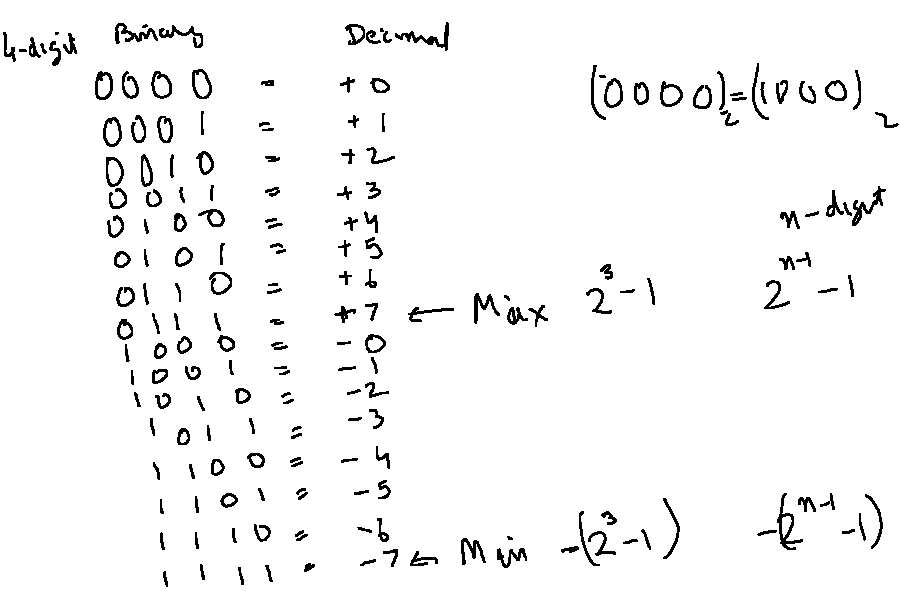
\includegraphics[width=12cm]{sign-magnitude-numbers.pdf}
\vspace{20em}

\subsection{One's complement negation}

You can convert a positive number (say +10) to negative number by applying a
negative sign in front of it (-(+10) = -10). It is more evident from taking
negative of a negative number (-(-10) = +10). In case of sign-magnitude
representation, the ``negative operator'' flips the sign bit. The next two
signed number representations (1's complement and 2's complement) are designed
around specific negative operator definitions.

\noindent Negate $13_{10} = 01101_2$ using 5-bit one's complement.
\vspace{10em}

\noindent Negate $-13_{10}$ using 5-bit one's complement.
\vspace{10em}

\subsection{One's complement binary numbers}

In one's complement representation, the negative operation is obtained by flipping
all the bits of the binary number. Example, a 5-bit one's
complement of $+10 = (01010)_2$ is $(10101)_2 = -10$. Note that flipping bits is
equivalent to subtracting the number from $(11111)_2$, hence the name. You can
also confirm that double negative operator yields back the same number.

\begin{prob}
  \begin{itemize}
  \item Write down all possible 4-digit binary numbers and corresponding decimal
    values if they are in sign magnitude format? What is the minimum and maximum value?
  \item What is the minimum and maximum value of n-digit signed binary number in
    one's complement?
  \end{itemize}
\end{prob}
\vspace{20em}

\begin{prob}
  Determine the decimal values of the following 1’s complement 6-digit binary numbers :
  \begin{enumerate}
  \item 01101110
  \item 10101101
  \end{enumerate}
\end{prob}
\vspace{20em}

\begin{prob}
  Convert the decimal numbers -17 and +23 into the 6-digit one's complement binary numbers and try adding them. What
  adjustments will you need to make to get the right result's (23-17=6) in binary representation.
\end{prob}
\vspace{20em}


\subsection{Two's complement negation}
In two's complement representation, the n-digit negative number is obtained by
subtracting the positive number from $2^{n}$. Example, two's
complement of 5-digit binary number $+10 = (01010)_2$ is $2^5 - 10 = 22 =
(11000)_2$. An easier algorithm to get two's complement goes via one's
complement. Note that $(11111)_2 = 2^5-1$. We can get two's complement by adding
1 to one's complement. To get two's complement:
\begin{enumerate}
\item Flip all the bits. (Same as taking one's complement).
\item Add 1 to the number.
\end{enumerate}

\noindent Negate $13_{10} = 01101_2$ using 5-bit two's complement.
\vspace{10em}

\noindent Negate $-13_{10}$ using 5-bit two's complement.
\vspace{10em}


How to convert one's complement number representation into sign-magnitude numbers?
\begin{enumerate}
\item Check if the number is positive or negative. Even for one's complement representation, or two's complement representation, if the MSB (Most-significant bit) is 1, then the number is negative, otherwise positive.
\item If positive: For positive numbers, two's complement, one's complement and sign magnitude are the same. No conversion between different representation is needed.
2.b If negative: For negative numbers. Flip the bits of 1's complement. Once you flip the 1's complement bits of a negative number, you get the corresponding positive number.
\item We still want to represent the original negative number. So we set the MSB of sign-magnitude representation to 1. Since the range (min and max) for both n-bit 1's complement and sign-magnitude are the same (between $-(2^{n-1}-1)$ and $2^{n-1}-1$), you can always represent 8-bit 1's complement numbers with needing to extend the 8-bit number to 9-bits.
\end{enumerate}

Example: Convert 8-bit one's complement 10101010 to 8-bit sign-magnitude
Let number n = 10101010
\begin{enumerate}
\item Is the number +ve or -ve: It is negative because it starts with 1.
\item The number is not positive.
\item Take the 1's complement of the negative number to get the positive part. i.e. Flip the bits:\\
-n = 01010101 or n = -(01010101)
\item
 We got the positive part of the number, but we want to represent the original negative number, so we set the MSB bit one. Hence, the equivalent sign-magnitude representation is:\\
n = 11010101
\end{enumerate}


\subsection{Two's complement representation}

% \begin{prob}
%   \begin{itemize}
%   \item Write down all possible 4-digit binary numbers and corresponding decimal
%     values if they are in two's complement format? What is the minimum and maximum value?
%   \item What is the minimum and maximum value of n-digit signed binary number in
%     two's complement?
%   \end{itemize}
% \end{prob}
\vspace{20em}

\begin{prob}
  Determine the decimal values of the following 2’s complement 6-digit numbers :
  \begin{enumerate}
  \item 01011110
  \item 10010111
  \end{enumerate}
\end{prob}
\vspace{10em}

\begin{prob}
  Convert the decimal numbers -17 and +23 into the 6-digit two's complement binary numbers and try adding them. What adjustments will you need to make to get the right result's (23-17=6) in binary representation.
\end{prob}
\vspace{20em}

\begin{prob}
  Convert the decimal numbers 73, 23, -17, and -163 into signed 8-bit numbers in the
  following representations:
  \begin{enumerate}
    \item Sign and magnitude
    \item 1’s complement
    \item 2’s complement
  \end{enumerate}
\end{prob}
\vspace{20em}


\subsection{Arithmetic overflow}
\begin{prob}
  Consider addition of 4-digit two's complement binary numbers
  \begin{enumerate}
  \item $1010_2 + 1101_2$
  \item $1011_2 + 1100_2$
  \end{enumerate}
  In which of the two case overflow happens? Can you come up with a rule to ``easily'' detect overflow?
\end{prob}
\vspace{20em}

\subsubsection{Rules for detecting arithmetic overflow:}

\begin{enumerate}
  \item Adding numbers of different signs never produces an overflow.
  \item Adding numbers of the same sign may produce an overflow
    \begin{enumerate}
        \item Wrong approach: Adding two negative 2's complement numbers always produces an additional carry-over 1, but that in itself isn't an overflow. An example, the range of 4-bit 2's complement numbers is between -8 to +7. Adding -3 to -4 in 2's complement is 1101 + 1100 produces an additional carry over 1. You can ignore the additional carry-over 1 to get the correct answer 1001 = -7 which is within range -8 to 7.
        \item Approach 1: The easiest way for now to detect overflow is if adding two -ve numbers results in a +ve number, or adding +ve numbers results in a -ve number.
        \item Approach 2: You can also do a range test in decimal based range test. The range of n-bit 2's complement numbers is between $-2^{n-1}$ and $2^{n-1}-1$. For 5-bit 2's complement numbers, it is between -16 and 15. For 6-bit 2's complement numbers, it is between -32 and 31.
        \item Approach 3: You can also check the carry-overs of the most significant two bits. If they match, i.e. 0 and 0, or 1 and 1, then there is no overflow. If they do not match, i.e. 0 and 1 or 1 and 0, then there is an overflow.
     \end{enumerate}
\end{enumerate}



\section{Binary coded decimal}
In Binary coded decimal (BCD), each decimal digit is represented by 4 bits. For
example, $1047 = (0001\_0000\_0100\_0111)_{\text{BCD}}$. It is useful in
input-output applications where the number has to be either displayed as decimal
or received as decimal.

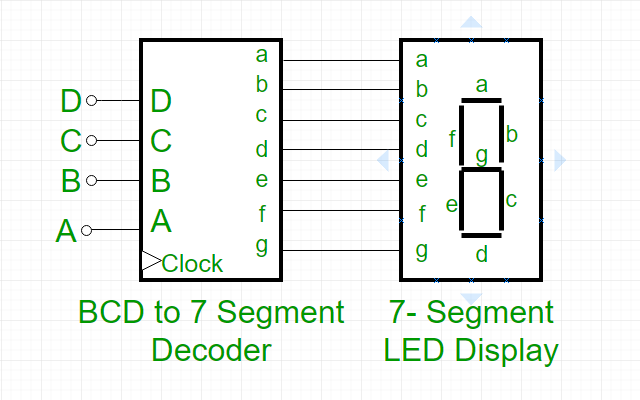
\includegraphics[width=0.5\linewidth]{bcdto7seg.png}

\begin{prob}
  Convert 11, 23, 35, 57 and 103897 to BCD?
\end{prob}
\vspace{10em}

\section{Gray code}
A sequence of binary numbers where only one bit changes when the number
increases by 1. It is helpful in applications like wheel encoders

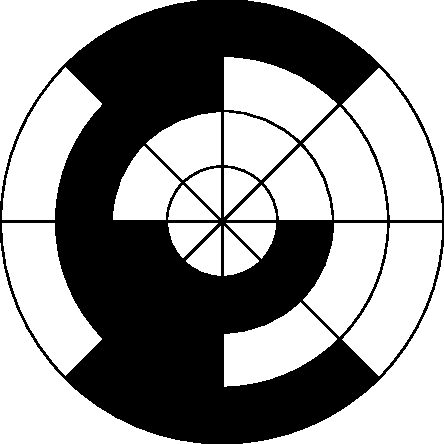
\includegraphics[width=0.5\linewidth]{gray-code.pdf}

\begin{prob}
  Write all possible 3-bit binary numbers in gray-code
\end{prob}
\vspace{10em}

\chapter{Boolean Algebra}
\maketitle
\section{Learning objectives}
\begin{enumerate}
\item Representing digital circuits
\item Converting between different notations: Boolean expression, logic
  networks and switching circuits
\item Converting between different logic network specifications: truth table, minterm,
  maxterms, product of sums canonical form and sum of product canonical form.
\end{enumerate}

\newpage
\section{Basic Gates and notations summary}
\rotatebox[origin=c]{90}{
\begin{tabular}{lccp{0.2\linewidth}ccc}
  \toprule
  Name & C/Verilog & Boolean expr. & Truth Table & Switching circuit & (ANSI) symbol & Venn diagram  \\
  \midrule
  AND Gate &
  \texttt{L = x1 \& x2} &
  $L = x_1 \cdot x_2 = x_1 x_2$ &
 \mbox{\begin{tabular}{cc|c}
 \toprule
 $x_1$ & $x_2$ & $x_1 \cdot x_2$ \\
 \midrule
 0 & 0 & 0 \\
 0 & 1 & 0 \\
 1 & 0 & 0 \\
 1 & 1 & 1 \\
 \bottomrule
 \end{tabular}} &
\includegraphics[width=0.2\linewidth]{AND-circuit.png} &
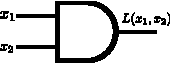
\includegraphics[width=0.2\linewidth]{AND_ANSI.pdf} &
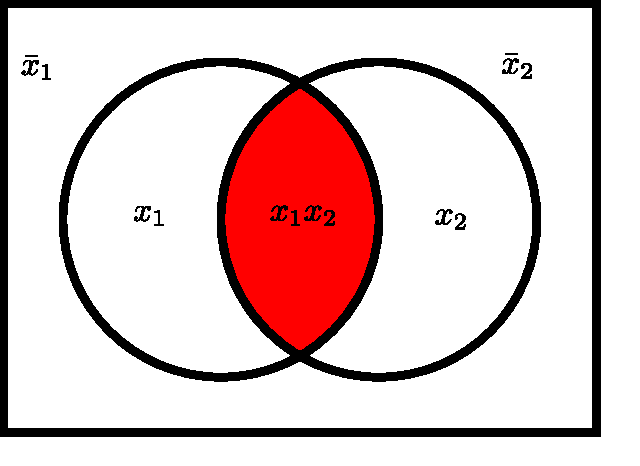
\includegraphics[width=0.2\linewidth]{AND_Venn.pdf}\\
  OR Gate &
\texttt{L = x1 | x2} &
$L = x_1 + x_2$ &
\mbox{\begin{tabular}{cc|c}
  \toprule
  $x_1$ & $x_2$ & $x_1 + x_2$ \\
  \midrule
  0 & 0 & 0 \\
  0 & 1 & 1 \\
  1 & 0 & 1 \\
  1 & 1 & 1 \\
  \bottomrule
\end{tabular}} &
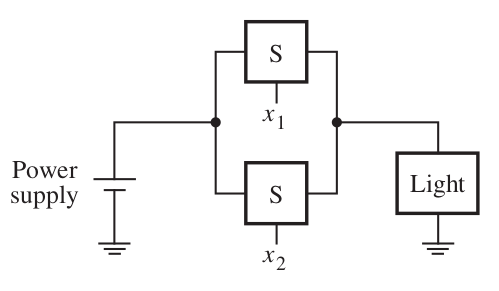
\includegraphics[width=0.2\linewidth]{OR-circuit.png} &
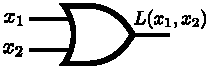
\includegraphics[width=0.2\linewidth]{OR_ANSI.pdf} & 
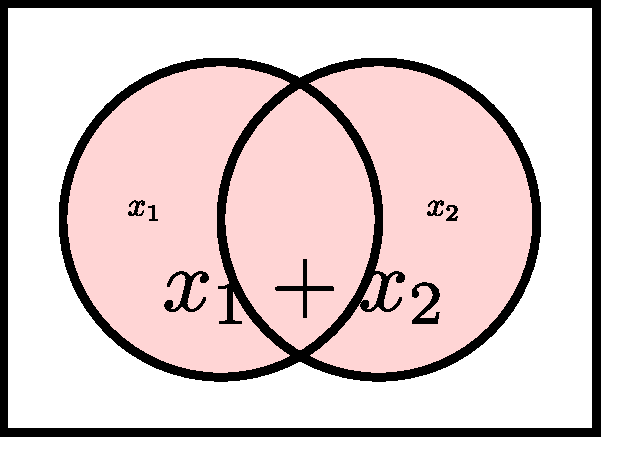
\includegraphics[width=0.2\linewidth]{OR_Venn.pdf}\\
  NOT Gate &
  \texttt{L = $\sim$ x1} &
$ L = \bar{x}_1 = x'_1$ &
\mbox{\begin{tabular}{c|c}
\toprule
$x_1$ & $\bar{x}_1$ \\
\midrule
0 & 1 \\
1 & 0 \\
\bottomrule
\end{tabular}} &
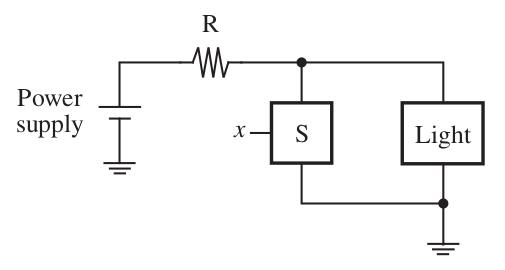
\includegraphics[width=0.2\linewidth]{NOT-circuit.png} &
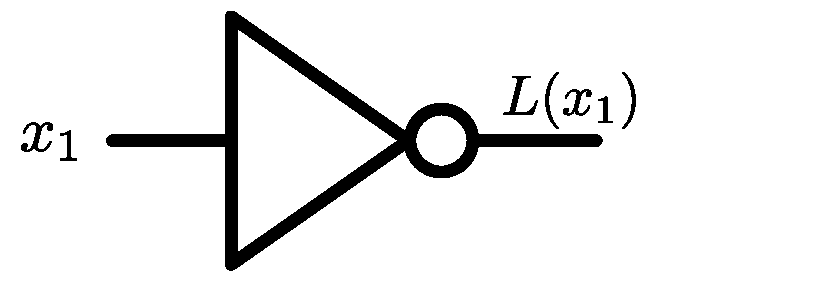
\includegraphics[width=0.2\linewidth]{NOT_ANSI.pdf} &
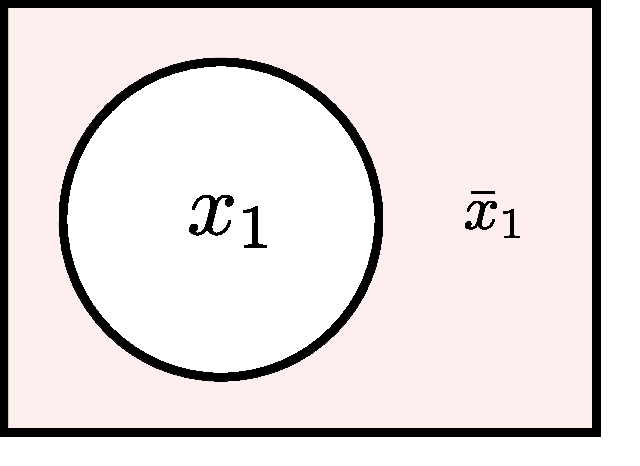
\includegraphics[width=0.2\linewidth]{NOT_Venn_x1.pdf}
\end{tabular}
}
\newpage

\section{Digital circuits or networks}

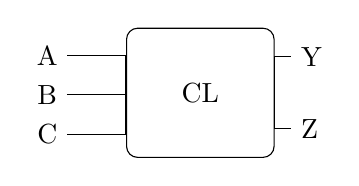
\begin{tikzpicture}[circuit logic US]
    \node (A) at (0,1) {A} ;
    \node (B) at (0,0.5) {B} ;
    \node (C) at (0,0) {C} ;
    \node [draw,rounded corners,inner sep=7mm,anchor=south west] (CL) at (1, -3mm) {CL} ; 
    \node [above right=3mm of CL.east] (Y) {Y} ;
    \node [below right=3mm of CL.east] (Z) {Z} ;

    \draw (A) -| (CL.west);
    \draw (B) -| (CL.west);
    \draw (C) -| (CL.west);
    \draw (CL.east) |- (Y);
    \draw (CL.east) |- (Z);
\end{tikzpicture}

\[
  Y = F(A, B, C) \qquad Z = G(A, B, C)
  \]

\section{Two input networks}
\begin{example}
  Convert the following (ANSI) network into a Boolean expression, a truth table
  and a Venn diagram.

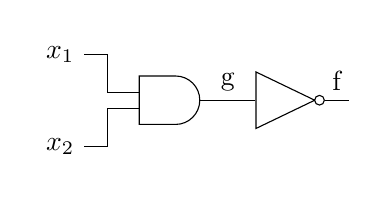
\begin{tikzpicture}[circuit logic US]
  \matrix[column sep=7mm]{
    \node (i1) {$x_1$}; & &  \\
    & \node [and gate] (a) {}; & \node [not gate] (n) {};\\
    \node (i2) {$x_2$}; & &  \\
  };
  \draw (i1.east) -- ++(right:3mm) |- (a.input 1);
  \draw (i2.east) -- ++(right:3mm) |- (a.input 2);
  \draw (a.output) to [edge label=g] (n.input);
  \draw (n.output) to [edge label=f] ++(right:3mm);
\end{tikzpicture}
\end{example}
\vspace{10em}

\begin{example}
  Convert the following Boolean expression into a (ANSI) network, a truth
  table and a Venn diagram:\\
  \[ f = \overline{x_1 + x_2}\]
\end{example}
\vspace{10em}

\begin{prob}
  Convert the following (ANSI) network into a Boolean expression, a truth table
  and a Venn diagram.

 \noindent 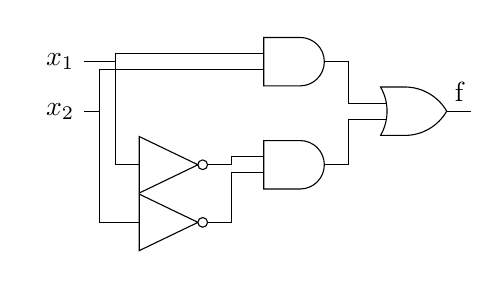
\begin{tikzpicture}[circuit logic US]
    \matrix[column sep=7mm]{
      \node (i1) {$x_1$}; & & \node [and gate] (x1nx2) {}; & \\
      \node (i2) {$x_2$}; &  &  &  \node [or gate] (f) {}; \\
       & \node [not gate] (n1) {}; & \node [and gate] (nx1x2) {};&  \\
      & \node [not gate] (n2) {}; &  & \\
    };
    \draw (i1.east) -- ++(right:4mm) |- (n1.input);
    \draw (i2.east) -- ++(right:2mm) |- (n2.input);

    \draw (i1.east) -- ++(right:4mm) |- (x1nx2.input 1);
    \draw (i2.east) -- ++(right:2mm) |- (x1nx2.input 2);

    \draw (n1.output) -- ++(right:3mm) |- (nx1x2.input 1);
    \draw (n2.output) -- ++(right:3mm) |- (nx1x2.input 2);

    \draw (x1nx2.output) -- ++(right:3mm) |- (f.input 1);
    \draw (nx1x2.output) -- ++(right:3mm) |- (f.input 2);

    \draw (f.output) to [edge label=f] ++(right:3mm);
  \end{tikzpicture}
\end{prob}
\vspace{10em}

\begin{example}
  Convert the following Boolean expression into a network, a truth
  table and a Venn diagram:\\
  \[ f = x_1 \bar{x}_2 + \bar{x}_1 x_2 \]
\end{example}
\vspace{20em}

\begin{prob}
Can two different circuits have the same truth table? Can two different truth tables
have the same circuit? Consider the following two circuits for example \\
\noindent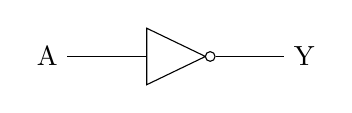
\begin{tikzpicture}[circuit logic US]
  \node (A) {A}; \node [not gate, right=of A] (notA) {}; \node [right=of notA] (Y) {Y};
  \draw (A) -- (notA.input);
  \draw (notA.output) -- (Y);
\end{tikzpicture}\\[1em]

\noindent\begin{tikzpicture}[circuit logic US]
  \node (A) {A}; \node [not gate, right=of A] (notA1) {};
  \draw (A) -- (notA.input);

  \node [not gate, right=of notA1] (notA2) {};
  \draw (notA1.output) -- (notA2.input);

  \node [not gate, right=of notA2] (notA3) {};
  \draw (notA2.output) -- (notA3.input);

  \node [right=of notA3] (Y) {Y};
  \draw (notA3.output) -- (Y);
\end{tikzpicture}

How about Venn digrams?
\end{prob}
\vspace{10em}

\begin{remark}
  Truth tables and Venn diagrams define \emph{what} the combinational circuit should do. Truth tables
  define output for every input.
  Boolean expression and networks define \emph{how} to achieve the desired input
  output relationship.
\end{remark}


\section{Multi-input networks}
\begin{example}
  Convert the following (ANSI) network into a Boolean expression and a truth table.
  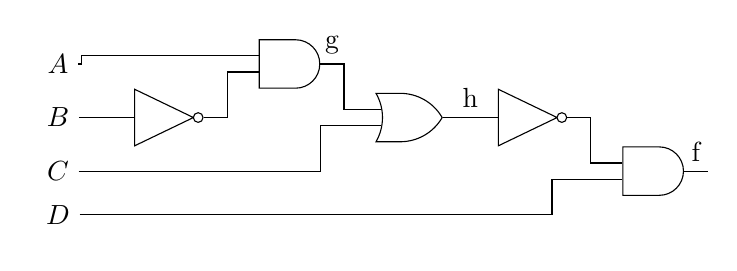
\begin{tikzpicture}[circuit logic US]
    \matrix[column sep=7mm]{
      \node (A) {$A$}; & &  \node [and gate] (andAB) {}; & & & \\
      \node (B) {$B$}; & \node [not gate] (nB) {};  &  & \node [or gate] (orGC) {}; & \node [not gate] (notH) {}; & \\
      \node (C) {$C$}; & & \node (C2) {}; & & & \node [and gate] (andHD) {}; \\
      \node (D) {$D$}; & &  & & \node (D2) {}; &\\
    };
    \draw (A) -- ++(right:3mm) |- (andAB.input 1);
    \draw (B) -- (nB.input);
    \draw (nB.output) -- ++(right:3mm) |- (andAB.input 2);

    \draw (andAB.output) to [edge label=g] ++(right:3mm) |- (orGC.input 1);
    \draw (C) -- (C2.east) -- ++(right:3mm) |- (orGC.input 2);

    \draw (orGC.output)  to [edge label=h] (notH.input);

    \draw (notH.output) -- ++(right:3mm) |- (andHD.input 1);
    \draw (D) -- (D2.east) -- ++(right:3mm) |- (andHD.input 2);
    
    \draw (andHD.output) to [edge label=f] ++(right:3mm);
  \end{tikzpicture}
\end{example}
\vspace{20em}

\begin{prob}
  Convert the following (ANSI) network into a Boolean expression and a truth table.
  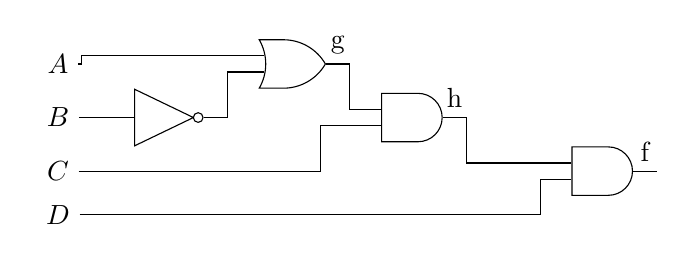
\begin{tikzpicture}[circuit logic US]
    \matrix[column sep=7mm]{
      \node (A) {$A$}; & &  \node [or gate] (andAB) {}; & & & \\
      \node (B) {$B$}; & \node [not gate] (nB) {};  &  & \node [and gate] (orGC) {}; &  & \\
      \node (C) {$C$}; & & \node (C2) {}; & & & \node [and gate] (andHD) {}; \\
      \node (D) {$D$}; & &  & & \node (D2) {}; &\\
    };
    \draw (A) -- ++(right:3mm) |- (andAB.input 1);
    \draw (B) -- (nB.input);
    \draw (nB.output) -- ++(right:3mm) |- (andAB.input 2);

    \draw (andAB.output) to [edge label=g] ++(right:3mm) |- (orGC.input 1);
    \draw (C) -- (C2.east) -- ++(right:3mm) |- (orGC.input 2);

    %\draw (orGC.output)  to [edge label=h] (andHD.input);

    \draw (orGC.output) to [edge label=h] ++(right:3mm) |- (andHD.input 1);
    \draw (D) -- (D2.east) -- ++(right:3mm) |- (andHD.input 2);
    
    \draw (andHD.output) to [edge label=f] ++(right:3mm);
  \end{tikzpicture}
\end{prob}
\vspace{20em}

\section{Minterms and Maxterms}
\subsection{Minterms}
Minterm is a product involving all inputs (or complements) to a function.
Every row of a truth table has a corresponding minterm.
Minterm is true if and only if the corresponding row in the table is active.

Minterms defined as follows for each row of a two input truth table:\\
\begin{tabular}{rrrp{20mm}}
  \toprule
  A & B &  minterm & minterm name\\
  \midrule
  0 & 0 &  $\bar{A} \bar{B}$ & $m_0$ \\
  0 & 1 &  $\bar{A}      B $ & $m_1$ \\
  1 & 0 &  $     A  \bar{B}$ & $m_2$ \\
  1 & 1 &  $     A       B $ & $m_3$ \\
  \bottomrule
\end{tabular}\\[1em]

\noindent Consider a two input circuit whose output $Y$ is given by the truth table:\\
\begin{tabular}{rrrrp{20mm}}
  \toprule
  A & B &  Y & minterm & minterm name\\
  \midrule
  0 & 0 & 0 & $\bar{A} \bar{B}$ & $m_0$ \\
  0 & 1 & 1 & $\bar{A}      B $ & $m_1$ \\
  1 & 0 & 0 & $     A  \bar{B}$ & $m_2$ \\
  1 & 1 & 1 & $     A       B $ & $m_3$ \\
  \bottomrule
\end{tabular}\\[1em]
then $Y = \bar{A}      B  + A B = m_1 + m_3 = \sum (1, 3)$.

\noindent This also gives the \emph{sum of products canonical form}.

\begin{example}
  What is the minterm $m_{13}$ for a 4-input circuit with inputs $x, y, z, w$
  (ordered from MSB to LSB).
\end{example}
\vspace{10em}

%\noindent Find the minterm $m_n$
%\begin{enumerate}
%    \item Convert the minterm number $n$ to a $m$-bit binary number where $m$ is the
%      order of inputs.
%    \item Replace 0 with the corresponding input complement and 1 with the input.
%\end{enumerate}

\begin{prob}
  What is the minterm $m_{23}$ for a 5-input circuit with inputs $a, b, c, d, e$
  (ordered from MSB to LSB).
\end{prob}
\vspace{10em}

\begin{example}
  Convert the following 4-input truth table into sum of minterms and sum of products canonical form.

  \noindent \begin{tabular}{p{20mm}llll|l}
    \toprule
    minterm name & A & B & C & D & f \\
    \midrule
    $m_0$ & 0 & 0 & 0 & 0 & 0 \\ 
    $m_1$ & 0 & 0 & 0 & 1 & 1 \\ 
    $m_2$ & 0 & 0 & 1 & 0 & 0 \\ 
    $m_3$ & 0 & 0 & 1 & 1 & 0 \\ 
    $m_4$ & 0 & 1 & 0 & 0 & 0 \\ 
    $m_5$ & 0 & 1 & 0 & 1 & 1 \\ 
    $m_6$ & 0 & 1 & 1 & 0 & 0 \\ 
    $m_7$ & 0 & 1 & 1 & 1 & 0 \\ 
    $m_8$ & 1 & 0 & 0 & 0 & 0 \\ 
    $m_9$ & 1 & 0 & 0 & 1 & 0 \\ 
    $m_{10}$ & 1 & 0 & 1 & 0 & 0 \\
    $m_{11}$ & 1 & 0 & 1 & 1 & 0 \\
    $m_{12}$ & 1 & 1 & 0 & 0 & 0 \\
    $m_{13}$ & 1 & 1 & 0 & 1 & 1 \\
    $m_{14}$ & 1 & 1 & 1 & 0 & 0 \\
    $m_{15}$ & 1 & 1 & 1 & 1 & 0 \\
    \bottomrule
  \end{tabular}
\end{example}

\begin{prob}
  Convert the following 4-input truth table into sum of minterms and sum of products canonical form.

  \noindent
  \begin{tabular}{p{20mm}llll|l}
    \toprule
    minterm name & A & B & C & D & f \\
    \midrule
    $m_0$ & 0 & 0 & 0 & 0 & 0 \\ 
    $m_1$ & 0 & 0 & 0 & 1 & 0 \\ 
    $m_2$ & 0 & 0 & 1 & 0 & 0 \\ 
    $m_3$ & 0 & 0 & 1 & 1 & 1 \\ 
    $m_4$ & 0 & 1 & 0 & 0 & 0 \\ 
    $m_5$ & 0 & 1 & 0 & 1 & 0 \\ 
    $m_6$ & 0 & 1 & 1 & 0 & 0 \\ 
    $m_7$ & 0 & 1 & 1 & 1 & 1 \\ 
    $m_8$ & 1 & 0 & 0 & 0 & 0 \\ 
    $m_9$ & 1 & 0 & 0 & 1 & 0 \\ 
    $m_{10}$ & 1 & 0 & 1 & 0 & 0 \\
    $m_{11}$ & 1 & 0 & 1 & 1 & 1 \\
    $m_{12}$ & 1 & 1 & 0 & 0 & 0 \\
    $m_{13}$ & 1 & 1 & 0 & 1 & 1 \\
    $m_{14}$ & 1 & 1 & 1 & 0 & 1 \\
    $m_{15}$ & 1 & 1 & 1 & 1 & 0 \\
    \bottomrule
  \end{tabular}
\end{prob}


\subsection{Maxterms}
Maxterm is a sum involving all inputs (or complements) to a function.
Every row of a truth table has a corresponding maxterm.
Minterm is false if and only if the corresponding row in the table is active.

Maxterms are defined as follows for each row of a two input truth table:\\
\begin{tabular}{rrrp{20mm}}
  \toprule
  A & B &  maxterm & maxterm name\\
  \midrule
  0 & 0 &  $A + B$ & $M_0$ \\
  0 & 1 &  $A + \bar{B} $ & $M_1$ \\
  1 & 0 &  $\bar{A} + B$ & $M_2$ \\
  1 & 1 &  $\bar{A} + \bar{B} $ & $M_3$ \\
  \bottomrule
\end{tabular}\\[1em]

\noindent Consider a two input circuit whose output $Y$ is given by the truth table:\\
\begin{tabular}{rrrrp{20mm}}
  \toprule
  A & B &  Y & maxterm & maxterm name\\
  \midrule
  0 & 0 &  0 & $A + B$ & $M_0$ \\
  0 & 1 &  1 & $A + \bar{B} $ & $M_1$ \\
  1 & 0 &  0 & $\bar{A} + B$ & $M_2$ \\
  1 & 1 &  1 & $\bar{A} + \bar{B} $ & $M_3$ \\
  \bottomrule
\end{tabular}\\[1em]
then $Y = (A+B)(\bar{A} + B) = M_0M_2$.

\noindent Writing a functional specification in terms of minterms is also called
product of sums canonical form.

\begin{example}
  Write the maxterm $M_{11}$ for 4-input Boolean function with the ordered inputs $A, B, C, D$.
\end{example}

% \noindent Find the maxterm $M_n$
% \begin{enumerate}
% \item Convert the maxterm number $n$ to a $m$-bit binary number where $m$ is the
%   order of inputs.
% \item Replace 0 with the corresponding input and 1 with the input complement.
% Add + between each input.
% \end{enumerate}

\begin{example}
  Convert the following 4-input truth table into product of maxterms and product of sums canonical form.

  \noindent
  \begin{tabular}{p{20mm}llll|l}
    \toprule
    maxterm name & A & B & C & D & f \\
    \midrule
    $M_0$ & 0 & 0 & 0 & 0 & 0 \\ 
    $M_1$ & 0 & 0 & 0 & 1 & 0 \\ 
    $M_2$ & 0 & 0 & 1 & 0 & 0 \\ 
    $M_3$ & 0 & 0 & 1 & 1 & 1 \\ 
    $M_4$ & 0 & 1 & 0 & 0 & 0 \\ 
    $M_5$ & 0 & 1 & 0 & 1 & 0 \\ 
    $M_6$ & 0 & 1 & 1 & 0 & 0 \\ 
    $M_7$ & 0 & 1 & 1 & 1 & 1 \\ 
    $M_8$ & 1 & 0 & 0 & 0 & 0 \\ 
    $M_9$ & 1 & 0 & 0 & 1 & 0 \\ 
    $M_{10}$ & 1 & 0 & 1 & 0 & 0 \\
    $M_{11}$ & 1 & 0 & 1 & 1 & 1 \\
    $M_{12}$ & 1 & 1 & 0 & 0 & 0 \\
    $M_{13}$ & 1 & 1 & 0 & 1 & 1 \\
    $M_{14}$ & 1 & 1 & 1 & 0 & 1 \\
    $M_{15}$ & 1 & 1 & 1 & 1 & 0 \\
    \bottomrule
  \end{tabular}
\end{example}

\begin{prob}
  Convert the following 4-input truth table into product of maxterms and products of sums canonical form.

  \noindent
  \begin{tabular}{p{20mm}llll|l}
    \toprule
    maxterm name & A & B & C & D & f \\
    \midrule
    $M_0$ & 0 & 0 & 0 & 0 & 0 \\ 
    $M_1$ & 0 & 0 & 0 & 1 & 1 \\ 
    $M_2$ & 0 & 0 & 1 & 0 & 1 \\ 
    $M_3$ & 0 & 0 & 1 & 1 & 1 \\ 
    $M_4$ & 0 & 1 & 0 & 0 & 1 \\ 
    $M_5$ & 0 & 1 & 0 & 1 & 0 \\ 
    $M_6$ & 0 & 1 & 1 & 0 & 1 \\ 
    $M_7$ & 0 & 1 & 1 & 1 & 1 \\ 
    $M_8$ & 1 & 0 & 0 & 0 & 0 \\ 
    $M_9$ & 1 & 0 & 0 & 1 & 1 \\ 
    $M_{10}$ & 1 & 0 & 1 & 0 & 1 \\
    $M_{11}$ & 1 & 0 & 1 & 1 & 1 \\
    $M_{12}$ & 1 & 1 & 0 & 0 & 0 \\
    $M_{13}$ & 1 & 1 & 0 & 1 & 1 \\
    $M_{14}$ & 1 & 1 & 1 & 0 & 1 \\
    $M_{15}$ & 1 & 1 & 1 & 1 & 0 \\
    \bottomrule
  \end{tabular}
\end{prob}

\begin{example}
  Write the 3-input truth table for the function $f = m_2 + m_3 + m_7$.
\end{example}
\vspace{10em}

\begin{prob}
  Write the 3-input truth table for the function $f = M_4M_5M_7$. 
\end{prob}
\vspace{10em}

\begin{prob}
  Write the truth table for the function $f = \bar{A}B\bar{C} + AB\bar{C}$. 
\end{prob}
\vspace{10em}

\section{Karnaugh maps}

\subsection{Two input K-maps}
\begin{Karnaughquatre}
  \phminterms{0,1,2,3}
\end{Karnaughquatre}

% \begin{example}
%   Convert the following truth table into a K-map.
% 
%   \noindent
%   \begin{tabular}{ll|l}
%     \toprule
%      A & B & f \\
%     \midrule
%     0 & 0 & 0 \\ 
%     0 & 1 & 1 \\ 
%     1 & 0 & 1 \\ 
%     1 & 1 & 0 \\ 
%     \bottomrule
%   \end{tabular}
% \end{example}
% \vspace{10em}

% \begin{prob}
%   Convert the following Venn Diagram into a K-map.
% 
%   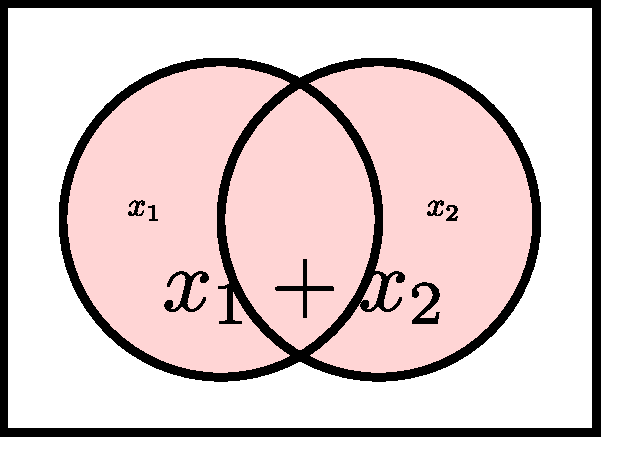
\includegraphics[width=0.2\linewidth]{OR_Venn.pdf}
% \end{prob}
% \vspace{10em}
  
\subsection{Three input K-maps}

\begin{Karnaughvuit}
  \phminterms{0,1,2,3,4,5,6,7}
\end{Karnaughvuit}

% \begin{prob}
%   Draw a K-map for the function $f = \bar{A}\bar{B}C + AB\bar{C}$.
% \end{prob}
% \vspace{10em}

\subsection{Four input K-maps}
\begin{Karnaugh}{AB}{CD}
  \phminterms{0,1,2,3,4,5,6,7,8,9,10,11,12,13,14,15}
\end{Karnaugh}


% \begin{prob}
%   Draw a K-map for a 4-input function $f = m_1 + m_2 + m_7 $.
% \end{prob}
% \vspace{10em}

\subsection{Five input K-maps}

A = 0
\begin{Karnaugh}{BC}{DE}
  \phminterms{0,1,2,3,4,5,6,7,8,9,10,11,12,13,14,15}
\end{Karnaugh} \hfill
A = 1
\begin{Karnaugh}{BC}{DE}
  \phmintermssixt{0,1,2,3,4,5,6,7,8,9,10,11,12,13,14,15}
\end{Karnaugh}

% \begin{prob}
%   Draw a K-map for a 5-input function $f = M_1 M_2 M_7 $.
% \end{prob}
% \vspace{10em}
\section{More Gates and notations summary}
\rotatebox[origin=c]{90}{
\begin{tabular}{lccp{0.2\linewidth}cp{0.2\linewidth}}
  \toprule
  Name & C/Verilog & Boolean expr. & Truth Table & (ANSI) symbol & K-map \\
  \midrule
  NAND Gate &
  \texttt{Q = \~{}(x1 \& x2)} &
  $Q = \overline{x_1 \cdot x_2} = \overline{x_1 x_2}$ &
 \mbox{\begin{tabular}{cc|c}
 \toprule
 $x_1$ & $x_2$ & $\overline{x_1 \cdot x_2}$ \\
 \midrule
 0 & 0 & 1 \\
 0 & 1 & 1 \\
 1 & 0 & 1 \\
 1 & 1 & 0 \\
 \bottomrule
 \end{tabular}} &
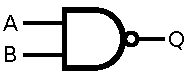
\includegraphics[width=0.2\linewidth]{NAND_ANSI_Labelled.pdf} &
\begin{minipage}[b][][t]{\linewidth}
\begin{Karnaughquatre}
\minterms{0,1,2}
\maxterms{3}
\end{Karnaughquatre}
\end{minipage}
\\
  NOR Gate &
\texttt{Q = \~{}(x1 | x2)} &
$Q = \overline{x_1 + x_2}$ &
\mbox{\begin{tabular}{cc|c}
  \toprule
  $x_1$ & $x_2$ & $\overline{x_1 + x_2}$ \\
  \midrule
  0 & 0 & 1 \\
  0 & 1 & 0 \\
  1 & 0 & 0 \\
  1 & 1 & 0 \\
  \bottomrule
\end{tabular}} &
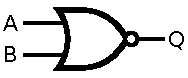
\includegraphics[width=0.2\linewidth]{NOR_ANSI_Labelled.pdf} & 
                                                               \begin{minipage}[b][][t]{\linewidth}
\begin{Karnaughquatre}
\minterms{3}
\maxterms{0,1,2}
\end{Karnaughquatre}
\end{minipage}
\\
XOR Gate &
\texttt{Q = x1 \^{} x2}
&
$ Q = x_1 \oplus x_2$
&
\mbox{\begin{tabular}{cc|c}
\toprule
$x_1$ & $x_2$ & $x_1 \oplus x_2$ \\
\midrule
0 & 0 & 0 \\
0 & 1 & 1 \\
1 & 0 & 1 \\
1 & 1 & 0 \\
\bottomrule
        \end{tabular}}
&
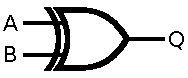
\includegraphics[width=0.2\linewidth]{XOR_ANSI_Labelled.pdf} &
\begin{minipage}[b][][t]{\linewidth}
\begin{Karnaughquatre}
\minterms{1,2}
\maxterms{0,3}
\end{Karnaughquatre}
\end{minipage}
\\
XNOR Gate &
\texttt{Q = \~{}(x1 \^{} x2)}
&
$ Q = \overline{x_1 \oplus x_2}$
&
\mbox{\begin{tabular}{cc|c}
        \toprule
        $x_1$ & $x_2$ & $\overline{x_1 \oplus x_2}$ \\
        \midrule
        0 & 0 & 1 \\
        0 & 1 & 0 \\
        1 & 0 & 0 \\
        1 & 1 & 1 \\
        \bottomrule
      \end{tabular}}
    &
    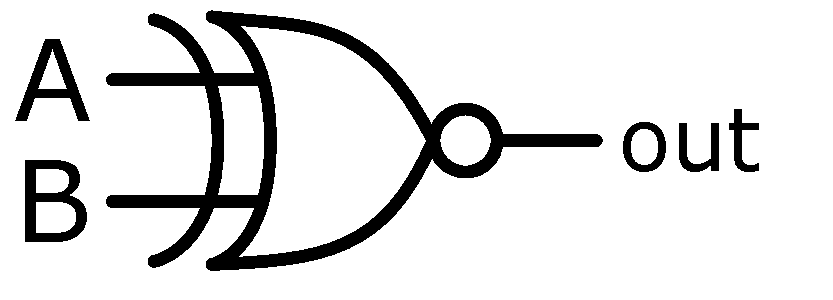
\includegraphics[width=0.2\linewidth]{XNOR_ANSI_Labelled.pdf} &
    \begin{minipage}[b][][t]{\linewidth}
      \begin{Karnaughquatre}
        \minterms{0,3}
        \maxterms{1,2}
      \end{Karnaughquatre}
    \end{minipage}
  \end{tabular}
}
\newpage


\begin{example}
  Convert the following Boolean expression into a K-map.
  $ f = \overline{A\bB + C}D $
\end{example}
\vspace{20em}

\begin{prob}
  Convert the following logic circuit into a K-map.\\
  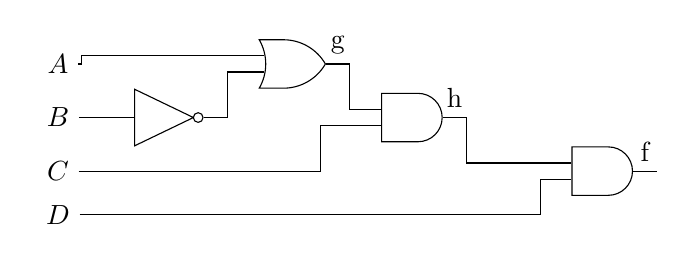
\begin{tikzpicture}[circuit logic US]
    \matrix[column sep=7mm]{
      \node (A) {$A$}; & &  \node [or gate] (andAB) {}; & & & \\
      \node (B) {$B$}; & \node [not gate] (nB) {};  &  & \node [and gate] (orGC) {}; &  & \\
      \node (C) {$C$}; & & \node (C2) {}; & & & \node [and gate] (andHD) {}; \\
      \node (D) {$D$}; & &  & & \node (D2) {}; &\\
    };
    \draw (A) -- ++(right:3mm) |- (andAB.input 1);
    \draw (B) -- (nB.input);
    \draw (nB.output) -- ++(right:3mm) |- (andAB.input 2);

    \draw (andAB.output) to [edge label=g] ++(right:3mm) |- (orGC.input 1);
    \draw (C) -- (C2.east) -- ++(right:3mm) |- (orGC.input 2);

    % \draw (orGC.output)  to [edge label=h] (andHD.input);

    \draw (orGC.output) to [edge label=h] ++(right:3mm) |- (andHD.input 1);
    \draw (D) -- (D2.east) -- ++(right:3mm) |- (andHD.input 2);
    
    \draw (andHD.output) to [edge label=f] ++(right:3mm);
  \end{tikzpicture}
\end{prob}
\vspace{20em}

\section{Boolean Algebra}

\subsection{Axioms of Boolean algebra}

\begin{enumerate}
\item 
  $ 0 \cdot 0 = 0 $
\item 
    $ 1 + 1 = 1 $
\item
    $ 1 \cdot 1 = 1 $
\item
    $ 0 + 0 = 0 $
\item
    $ 0 \cdot 1 = 1 \cdot 0 = 0 $
\item
      $ \bar{0} = 1 $
\item
        $ \bar{1} = 0 $
\item
      $ x = 0 \text{ if } x \ne 1$ 
    \item
      $ x = 1 \text{ if } x \ne 0$ 
\end{enumerate}

\subsection{Single variable theorems (Prove by drawing K-maps)}

\begin{enumerate}
\item $ x \cdot 0 = 0 $
  \vspace{5em}
\item $ x + 1 = 1 $
  \vspace{5em}
\item $ x \cdot 1 = x $
  \vspace{5em}
\item $ x + 0 = x $
  \vspace{5em}
\item $ x \cdot x = x $
  \vspace{5em}
\item $ x + x = x $
  \vspace{5em}
\item $ x \cdot \bar{x} = 0 $
  \vspace{5em}
\item $ x + \bar{x} = 1 $
  \vspace{5em}
\item $\bar{\bar{x}} = x $
  \vspace{5em}
\end{enumerate}

\begin{remark}[Duality]
  Swap $+$ with $\cdot$ and 0 with 1 to get another theorem
\end{remark}

\subsection{Two and three variable properties (Prove by K-maps)}

\begin{enumerate}
\item Commutative: $x\cdot y = y \cdot x$ , $x + y = y + x$
  \vspace{10em}
\item Associative: $x\cdot(y\cdot z) = (x \cdot y) \cdot z$, $x+(y+ z) = (x + y) + z$
  \vspace{10em}
\item Distributive: $x\cdot(y + z) = x \cdot y + x \cdot z$, $x + y \cdot z = (x + y) \cdot (y + z)$
  \vspace{10em}
\item Absorption: $x + x\cdot y = x$, $x \cdot (x+y) = x$
  \vspace{10em}
\item Combining: $x \cdot y + x \cdot \bar{y}$, $(x+y) \cdot (x + \bar{y}) = x$
  \vspace{10em}
\item DeMorgan's theorem: $\overline{x \cdot y} = \bar{x} + \bar{y}$,
  $\overline{x + y} = \bar{x} \cdot \bar{y}$.
  \vspace{10em}
\item Concensus:
  \begin{enumerate}
  \item $x + \bar{x}\cdot y = x + y$
    \vspace{10em}
  \item $x \cdot (\bar{x} + y) = x \cdot y$
    \vspace{10em}
  \item $x \cdot y + y\cdot z + \bar{x} \cdot z = x\cdot y + \bar{x} \cdot z$
    \vspace{10em}
  \item $(x + y) \cdot (y+ z) \cdot (\bar{x} + z) = (x+ y) \cdot (\bar{x} + z)$
    \vspace{10em}
  \end{enumerate}
\end{enumerate}

\begin{example}[Multiplexer]
  Multiplexer is a circuit used to select one of the input lines $x_1$ and $x_2$
  based only select input $s$. When $s=0$, $x_1$ is selected, $x_2$ is selected otherwise.
  Find a boolean expression and a circuit for multiplexer\\
  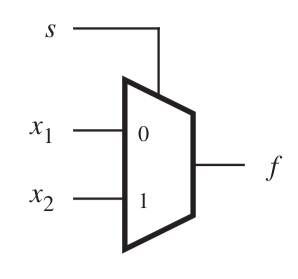
\includegraphics[width=0.2\linewidth]{multiplexer-symbol.png}
  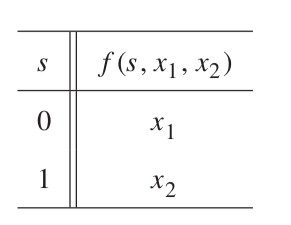
\includegraphics[width=0.2\linewidth]{multiplexer-spec.png}
\end{example}
\vspace{10em}

\begin{example}
  Simplify $f = \bA\bB\bC + A \bB\bC + A\bB\bC $ using boolean algebra.
\end{example}
\vspace{10em}

\begin{example}
  Simplify $f = \bA\bA\bC + \bA\bB C $ using K-maps.
\end{example}
\vspace{10em}
\section{Logic minimization}
\input{./0916-K-maps/0919-notes.tex}
\input{./0916-K-maps/0921-notes.tex}
\maketitle

\includegraphics[width=0.3\linewidth]{figures/K-map-flowchart.png}

%
\begin{example}
  \begin{Karnaugh}{AB}{CD}
    \minterms{4,5,7,6,8,9,10,13}
    \indeterminants{0,7,15}
  \end{Karnaugh}
\end{example}%
% 

\begin{prob}
  Find the minimum SOP (sum of products) and POS (product of sum) expression for
  the function $f(a,b,c,d) = \prod M(5, 7, 13, 14, 15) \cdot \prod D(1, 2, 3, 9)$
\end{prob}%
% 

\chapter{Adders, Muxes and Decoders}
\todo{Provide Verilog idioms for each of the sequential circuits}

\todo{The build up of SR latch is interesting from here.}
\url{https://www.youtube.com/watch?v=BYN8Zmk6HJY}

\todo{JK latch and T ff are not that interesting}

\todo{Metastability must be introduced}

\section{Objectives}
\begin{enumerate}
  \item Understand timing diagrams, gate delays and critical path
  \item Design Hazard-free two level circuits
  \item Building blocks of sequential circuits
  \item Analyze a sequential circuit and derive a state-table and a state-graph
  \item Derive a state graph or state table from a word description of the problem
  \item Understanding the structure of an FPGA
\end{enumerate}

\section{Why do we need sequential circuits?}

\begin{example}
  Think about this problem: Design an occupancy counter that depends on a
  sensor $S$ at the class door. The sensor is triggered every time a person passes
  through the door. The counter can be reset to zero with a reset button. Assume
  we only need up to two bit counter $C_1C_0$. Draw a truth table for this
  circuit. Do you have requisite knowledge for designing this circuit? Can this
  circuit be designed without a memory element?
\end{example}
\vspace{10em}


\section{Timing diagrams and propagation delays}

\begin{example}[Timing diagram]
  Draw a timing diagram for an ideal NAND gate.
\end{example}
\vspace{20em}

\subsection{Delays}
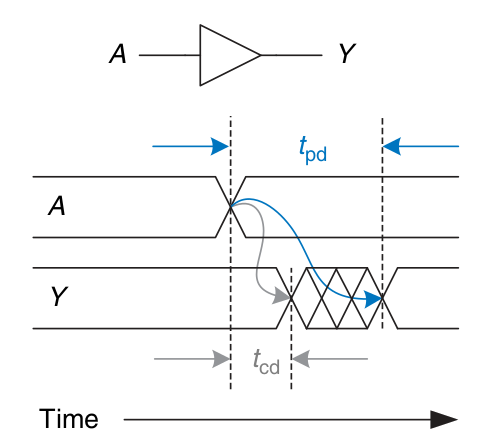
\includegraphics[width=0.5\linewidth]{fig/fig2.67-delays-tpd-tcd.png}
\begin{definition}[Propagation delay ($t_{pd}$)]
\end{definition}
\vspace{5em}

\begin{definition}[Contamination delay ($t_{cd}$)]
\end{definition}
\vspace{5em}

\subsection{Paths}
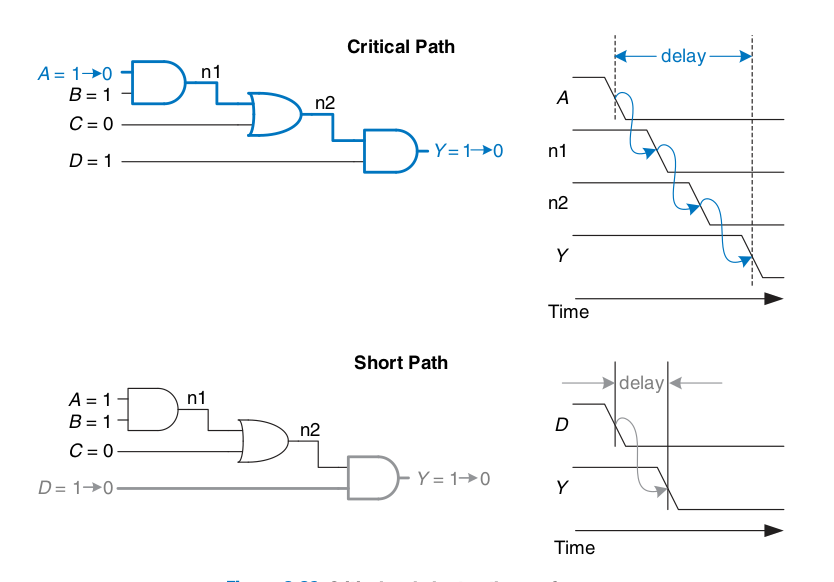
\includegraphics[width=0.8\linewidth]{fig/fig2.68-short-path-and-critical-path.png}
\begin{example}
  Find the propagation delay of the circuit above given that propagation delay
  of each gate is $100 ps$  add contamination delay of $60ps$.
\end{example}
\vspace{10em}

\section{Glitches or Hazards}
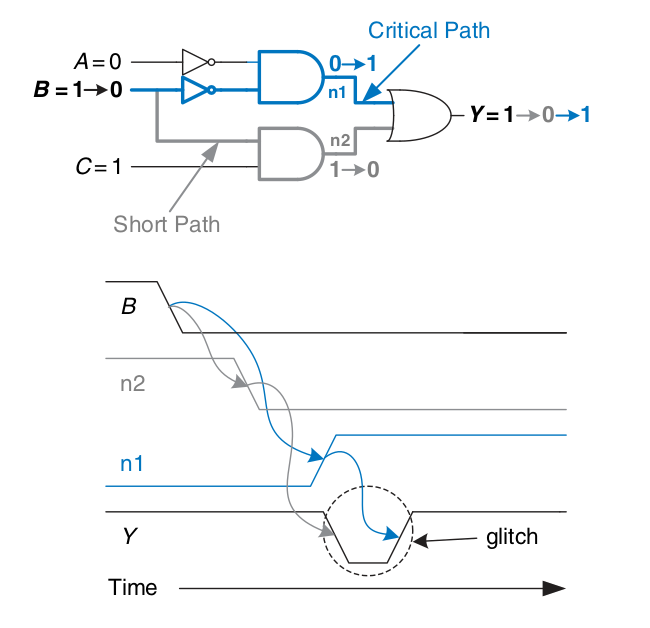
\includegraphics[width=0.6\linewidth]{fig/fig2.76-timing-of-a-glitch.png}
\begin{definition}[Glitch or Hazard]

\end{definition}
\vspace{5em}

\begin{example}
  Design a circuit that fixes the glitch in the above circuit (also known as
  glitch-free or hazard-free circuit).
\end{example}
\vspace{10em}


\section{How to create memory element from circuits}

Two types of memory
\begin{enumerate}
  \item Volatile memory. For example, RAM, CPU registers.
  \item Non-volatile memory. For example, SSD, Flash drives. (Not covered in this course)
    \begin{enumerate}
    \item Memories that require periodic refreshing. For example, DRAM: Dynamics Random Access memory (Not covered in this course)\\
      \includegraphics[width=0.6\linewidth]{./fig/DRAM-cell.png}~\footnote{Image
        source: \url{allaboutcircuits.com/technical-articles/introduction-to-dram-dynamic-random-access-memory/}}
    \item Memories that are always refreshing. For example, SRAM: Static Random
      Access memory~\cite[Appendix~B.64]{stephen2022fundamentals}\\
      \includegraphics[width=0.4\linewidth]{./fig/SRAM-cell.png}
    \end{enumerate}
\end{enumerate}

\section{Latches and Flip-Flops \cite[Sec~3.2]{harris2022digital}}

\begin{example}[Ring oscillator ] \cite[Sec~3.31]{harris2022digital}
  How many stable states does the following circuit have?\\
  \includegraphics[width=0.6\linewidth]{./fig/ring-oscillator.pdf} 
\end{example}
\vspace{10em}

\begin{definition}[Astable circuits]
\end{definition}
\vspace{5em}


\begin{example}
  Analyze the timing diagram of the following circuit.\\
  \includegraphics[width=0.4\linewidth]{./fig/simple-memory-element.png}
\end{example}
\vspace{10em}

\begin{definition}[Bistable circuits]
\end{definition}
\vspace{5em}

\begin{definition}[Characteristic or state table]
  Draw the characteristic or state table of the above circuit. 
\end{definition}
\vspace{10em}



\subsection{SR (Set-Reset) latch \cite[Sec~3.2.1]{harris2022digital}}

\begin{definition}[SR latch]
  The following circuit is called the SR latch. \\
  \includegraphics[width=0.3\linewidth]{./fig/fig3.3-SR-latch.png} \\
  \begin{enumerate}
    \item How many stable states does this circuit have?
    \item Draw its characteristic or state table.
    \item Draw SR latch symbol
  \end{enumerate}
\end{definition}
\vspace{20em}


\begin{prob}[SR latch using NAND gates]
Draw the characteristic or state table for the following circuit\\
  \includegraphics[width=0.3\linewidth]{./fig/fig3.65-SR-NAND-latch.png} \\
\end{prob}

\subsection{Gated SR latch \cite[Sec~5.2]{stephen2022fundamentals}}

\begin{definition}[Gated SR latch]
  The following circuit is called the Gated SR latch. \\
  \includegraphics[width=0.6\linewidth]{./fig/gated-SR-latch.png} \\
  \begin{enumerate}
  \item Draw its characteristic table.
  \item Draw the Gated SR latch symbol
  \end{enumerate}
\end{definition}
\vspace{20em}

\subsection{D (Data) latch \cite[Sec~3.2.2]{harris2022digital}}

\begin{definition}[D latch]
  The following circuit is called the D latch. \\
  \includegraphics[width=0.6\linewidth]{./fig/fig3.7-D-latch.png} \\
  \begin{enumerate}
  \item Draw its characteristic table.
  \item Draw the D latch symbol
  \end{enumerate}
\end{definition}
\vspace{20em}

\subsection{D flip-flop \cite[Sec~3.2.2]{harris2022digital}}

\begin{definition}[D flip-flop]
  The following circuit is called the D flip-flop. \\
  \includegraphics[width=0.6\linewidth]{./fig/fig3.8-D-flip-flop.png} \\
  \begin{enumerate}
  \item Draw its timing  diagram
  \item Draw its characteristic table.
  \item Draw the D flip-flop symbol
  \end{enumerate}
\end{definition}
\vspace{20em}

\begin{remark}
  What is the difference between a latch and a flip-flop?
\end{remark}
\vspace{5em}

\begin{example}
  Add a \emph{RESET} signal to the D flip-flop that resets the state of flip-flop to 0.
\end{example}
\vspace{20em}

\begin{example}
  The toggle (T) flip-flop has one input, CLK, and one output, Q. On
  each rising edge of CLK, Q toggles to the complement of its previous value. Draw
  a schematic for a T flip-flop using a D flip-flop and an inverter.
\end{example}
\vspace{20em}

\begin{prob}
  A JK flip-flop receives a clock and two inputs, J and K. On the rising
  edge of the clock, it updates the output, Q. If J and K are both 0, Q retains its old
  value. If only J is 1, Q becomes 1. If only K is 1, Q becomes 0. If both J and K are 1,
  Q becomes the opposite of its present state.
  \begin{enumerate}
  \item Construct a JK flip-flop using a D flip-flop and some combinational logic.
  \item Construct a D flip-flop using a JK flip-flop and some combinational logic.
  \item Construct a T flip-flop (see Exercise 3.9) using a JK flip-flop.
  \end{enumerate}
\end{prob}


\section{Finite State Machines~\cite[Sec~3.4]{harris2022digital}}\footnote{These
  notes will not fit on your note sheet.}

\begin{example}
  Design an occupancy counter that depends on a
  sensor $S$ at the class door. The sensor is triggered every time a person passes
  through the door. Assume that the counter starts at zero. Assume
  we only need up to two bit counter $C_1C_0$. Draw a state table for this
  circuit.
\end{example}

\begin{prob}
  A divide-by-N counter has one output and no inputs. The output Y is HIGH for
  one clock cycle out of every N. In other words, the output divides the frequency
  of the clock by N. The waveform for a divide-by-3 counter is shown here:\\
  \includegraphics[width=0.8\linewidth]{./fig/fig.38a-divide-by-3-counter.png}\\
  Sketch circuit designs for such a counter
\end{prob}

\begin{prob}
  Design a 3-bit counter which counts in the sequence:
  001, 011, 010, 110, 111, 100, (repeat) 001, ...
\end{prob}

\begin{example}
  Design an odd-even counter for an single bit input. The output of this circuit
  should be 1 if the number of 1s to the input have been odd so far and 0
  otherwise.
\end{example}

\begin{example}[Sequence detectors]
  A sequential circuit has one input and one output. The output becomes 1 and
  remain 1 thereafter when at least two 0's and at least two 1's have occurred
  as inputs regardless of the order of 
\end{example}

\begin{example}
  Consider the problem of inventing a controller for a traffic light at a busy
  intersection on campus. There are two traffic
  sensors, $T_A$ and $T_B$ , on Academic Ave. and Bravado Blvd., respectively.
  Each sensor indicates TRUE if students are present and FALSE if the
  street is empty. There are two traffic lights, $L_A$ and $L_B$, to control
  traffic. Each light receives digital inputs specifying whether it should be
  green, yellow, or red.
  When the system is reset, the lights are green on Academic Ave. and red on Bravado Blvd.
  As long as traffic is present on Academic Ave., the lights do not change. When there
  is no longer traffic on Academic Ave., the light on Academic Ave.
  becomes yellow for 5 seconds before it turns red and Bravado Blvd.’s light
  turns green. Similarly, the Bravado Blvd. light remains green as long as
  traffic is present on the boulevard, then turns yellow and eventually red.
  \\
  \includegraphics[width=0.5\linewidth]{./fig/fig3.23-campus-map.png}
  \includegraphics[width=0.5\linewidth]{./fig/fig3.24-traffic-light-controller.png}
  \begin{enumerate}
  \item Draw a state transition diagram
  \item Draw a state table 
  \item Assign binary encodings to each of the states
  \item Redraw the state table with binary encodings. Design a minimal SOP
    boolean expression.
  \item Assign binary encodings to each of the output and redraw the output
    table. Design a minimal SOP boolean expression for the outputs.
  \end{enumerate}
\end{example}


\begin{prob}
  Design a circuit for a 2x2 pixel resolution pong game, where the ball can only
  occupy 4 possible pixels and a single paddle occupies another 2 pixels. The
  ball bounces of the paddle when the paddle is in the correct row. To keep it
  interesting, the ball takes a different path from the source path. Track the
  score with a single bit counter.
\end{prob}

% \chapter{Review}
% \input{./0930-review/0919-notes.tex}
% \input{./0930-review/0921-notes.tex}
% \maketitle

\includegraphics[width=0.3\linewidth]{figures/K-map-flowchart.png}

%
\begin{example}
  \begin{Karnaugh}{AB}{CD}
    \minterms{4,5,7,6,8,9,10,13}
    \indeterminants{0,7,15}
  \end{Karnaugh}
\end{example}%
% 

\begin{prob}
  Find the minimum SOP (sum of products) and POS (product of sum) expression for
  the function $f(a,b,c,d) = \prod M(5, 7, 13, 14, 15) \cdot \prod D(1, 2, 3, 9)$
\end{prob}%
% 

% 

\section{Syllabus covered}
\begin{todolist}
  \item[\done] Binary numbers, Hexadecimal, Sign-magnitude, One's-complement and
    Two's complement. Conversions between them.
  \item[\done] Generate minterms, maxterms, SOP canonical form and POS
    canonical forms and convert between them\\
  \item[\done]  Understand and use the laws and theorems of Boolean Algebra
  \item[\done]  Perform algebraic simplification using Boolean algebra
  \item[\done]  Simplification using K-maps
  \item[\done]  Derive sum of product and product of sums expressions for a combinational circuit
  \item[\done]  Convert combinational logic to NAND-NAND and NOR-NOR forms
  \item[\done]  Simplification using Quine-McCluskey method, PI tables and Petrick's method
  \item  Design combinational circuits for positive and negative logic
  \item  Design Hazard-free two level circuits and understand Hazards in multi-level circuits
  \item Compute noise margin of one device
  \item Describe how tri-state and open-collector outputs are different from totem-pole outputs.
  \item Different between and limitations of master-slave and edge-triggered flip-flops.
  \item Compute fan out and noise margin of one device driving the same time
  \item Know the differences and similarities between PAL, PLA, and ROMs and can use each for logic design
  \item Design combinational circuits using multiplexers and decoders
  \item Analyze a sequential circuit and derive a state-table and a state-graph
  \item Understand the difference between synchronous and asynchronous inputs
  \item Derive a state graph or state table from a word description of the problem
  \item Reduce the number of states in a state table using row reduction and implication tables
  \item Perform a state assignment using the guideline method
  \item Implement a design using JK, SR, D or T flip-flops
  \item Analyse and design both Mealy and Moore sequential circuits with multiple inputs and multiple outputs
  \item Convert between Mealy and Moore designs
  \item Partition a system into multiple state machines
\end{todolist}

\subsection{Labs (not questioned in exams)}
\begin{todolist}
  \item Use computer tools to enter designs graphically and HDL
  \item Simulate designs using computer tools
  \item Use computer tools to program gate arrays logic and debug and test
\end{todolist}

\newpage

% \input{./0930-review/0930-sample-exam.tex}
\chapter{Sequential Logic}
\todo{Provide Verilog idioms for each of the sequential circuits}

\todo{The build up of SR latch is interesting from here.}
\url{https://www.youtube.com/watch?v=BYN8Zmk6HJY}

\todo{JK latch and T ff are not that interesting}

\todo{Metastability must be introduced}

\section{Objectives}
\begin{enumerate}
  \item Understand timing diagrams, gate delays and critical path
  \item Design Hazard-free two level circuits
  \item Building blocks of sequential circuits
  \item Analyze a sequential circuit and derive a state-table and a state-graph
  \item Derive a state graph or state table from a word description of the problem
  \item Understanding the structure of an FPGA
\end{enumerate}

\section{Why do we need sequential circuits?}

\begin{example}
  Think about this problem: Design an occupancy counter that depends on a
  sensor $S$ at the class door. The sensor is triggered every time a person passes
  through the door. The counter can be reset to zero with a reset button. Assume
  we only need up to two bit counter $C_1C_0$. Draw a truth table for this
  circuit. Do you have requisite knowledge for designing this circuit? Can this
  circuit be designed without a memory element?
\end{example}
\vspace{10em}


\section{Timing diagrams and propagation delays}

\begin{example}[Timing diagram]
  Draw a timing diagram for an ideal NAND gate.
\end{example}
\vspace{20em}

\subsection{Delays}
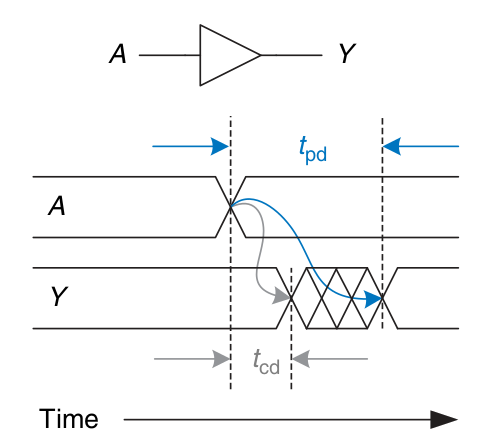
\includegraphics[width=0.5\linewidth]{fig/fig2.67-delays-tpd-tcd.png}
\begin{definition}[Propagation delay ($t_{pd}$)]
\end{definition}
\vspace{5em}

\begin{definition}[Contamination delay ($t_{cd}$)]
\end{definition}
\vspace{5em}

\subsection{Paths}
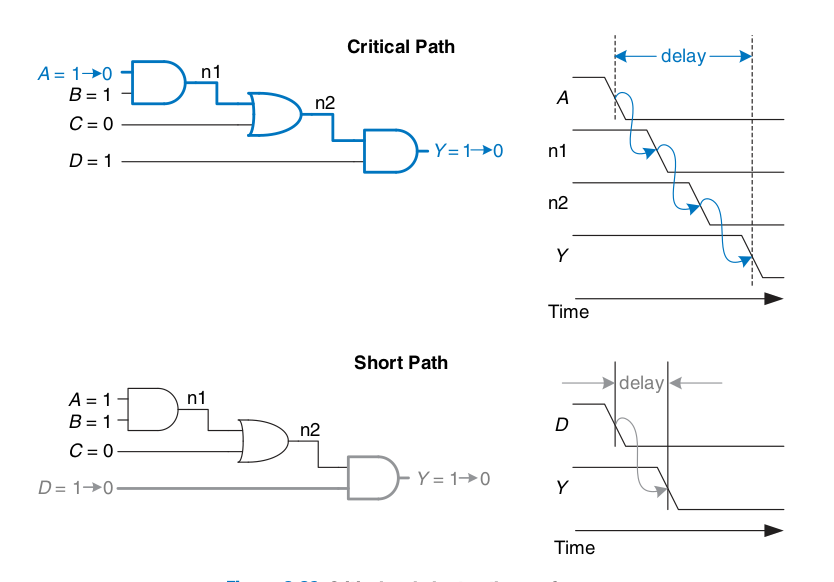
\includegraphics[width=0.8\linewidth]{fig/fig2.68-short-path-and-critical-path.png}
\begin{example}
  Find the propagation delay of the circuit above given that propagation delay
  of each gate is $100 ps$  add contamination delay of $60ps$.
\end{example}
\vspace{10em}

\section{Glitches or Hazards}
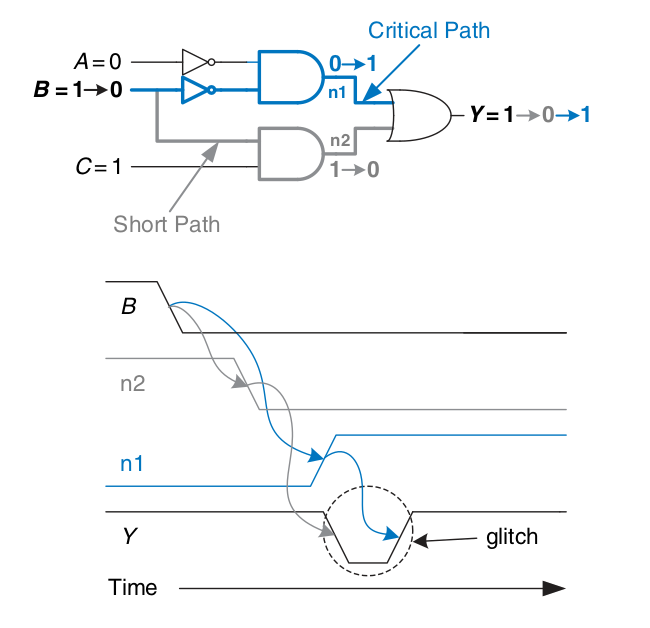
\includegraphics[width=0.6\linewidth]{fig/fig2.76-timing-of-a-glitch.png}
\begin{definition}[Glitch or Hazard]

\end{definition}
\vspace{5em}

\begin{example}
  Design a circuit that fixes the glitch in the above circuit (also known as
  glitch-free or hazard-free circuit).
\end{example}
\vspace{10em}


\section{How to create memory element from circuits}

Two types of memory
\begin{enumerate}
  \item Volatile memory. For example, RAM, CPU registers.
  \item Non-volatile memory. For example, SSD, Flash drives. (Not covered in this course)
    \begin{enumerate}
    \item Memories that require periodic refreshing. For example, DRAM: Dynamics Random Access memory (Not covered in this course)\\
      \includegraphics[width=0.6\linewidth]{./fig/DRAM-cell.png}~\footnote{Image
        source: \url{allaboutcircuits.com/technical-articles/introduction-to-dram-dynamic-random-access-memory/}}
    \item Memories that are always refreshing. For example, SRAM: Static Random
      Access memory~\cite[Appendix~B.64]{stephen2022fundamentals}\\
      \includegraphics[width=0.4\linewidth]{./fig/SRAM-cell.png}
    \end{enumerate}
\end{enumerate}

\section{Latches and Flip-Flops \cite[Sec~3.2]{harris2022digital}}

\begin{example}[Ring oscillator ] \cite[Sec~3.31]{harris2022digital}
  How many stable states does the following circuit have?\\
  \includegraphics[width=0.6\linewidth]{./fig/ring-oscillator.pdf} 
\end{example}
\vspace{10em}

\begin{definition}[Astable circuits]
\end{definition}
\vspace{5em}


\begin{example}
  Analyze the timing diagram of the following circuit.\\
  \includegraphics[width=0.4\linewidth]{./fig/simple-memory-element.png}
\end{example}
\vspace{10em}

\begin{definition}[Bistable circuits]
\end{definition}
\vspace{5em}

\begin{definition}[Characteristic or state table]
  Draw the characteristic or state table of the above circuit. 
\end{definition}
\vspace{10em}



\subsection{SR (Set-Reset) latch \cite[Sec~3.2.1]{harris2022digital}}

\begin{definition}[SR latch]
  The following circuit is called the SR latch. \\
  \includegraphics[width=0.3\linewidth]{./fig/fig3.3-SR-latch.png} \\
  \begin{enumerate}
    \item How many stable states does this circuit have?
    \item Draw its characteristic or state table.
    \item Draw SR latch symbol
  \end{enumerate}
\end{definition}
\vspace{20em}


\begin{prob}[SR latch using NAND gates]
Draw the characteristic or state table for the following circuit\\
  \includegraphics[width=0.3\linewidth]{./fig/fig3.65-SR-NAND-latch.png} \\
\end{prob}

\subsection{Gated SR latch \cite[Sec~5.2]{stephen2022fundamentals}}

\begin{definition}[Gated SR latch]
  The following circuit is called the Gated SR latch. \\
  \includegraphics[width=0.6\linewidth]{./fig/gated-SR-latch.png} \\
  \begin{enumerate}
  \item Draw its characteristic table.
  \item Draw the Gated SR latch symbol
  \end{enumerate}
\end{definition}
\vspace{20em}

\subsection{D (Data) latch \cite[Sec~3.2.2]{harris2022digital}}

\begin{definition}[D latch]
  The following circuit is called the D latch. \\
  \includegraphics[width=0.6\linewidth]{./fig/fig3.7-D-latch.png} \\
  \begin{enumerate}
  \item Draw its characteristic table.
  \item Draw the D latch symbol
  \end{enumerate}
\end{definition}
\vspace{20em}

\subsection{D flip-flop \cite[Sec~3.2.2]{harris2022digital}}

\begin{definition}[D flip-flop]
  The following circuit is called the D flip-flop. \\
  \includegraphics[width=0.6\linewidth]{./fig/fig3.8-D-flip-flop.png} \\
  \begin{enumerate}
  \item Draw its timing  diagram
  \item Draw its characteristic table.
  \item Draw the D flip-flop symbol
  \end{enumerate}
\end{definition}
\vspace{20em}

\begin{remark}
  What is the difference between a latch and a flip-flop?
\end{remark}
\vspace{5em}

\begin{example}
  Add a \emph{RESET} signal to the D flip-flop that resets the state of flip-flop to 0.
\end{example}
\vspace{20em}

\begin{example}
  The toggle (T) flip-flop has one input, CLK, and one output, Q. On
  each rising edge of CLK, Q toggles to the complement of its previous value. Draw
  a schematic for a T flip-flop using a D flip-flop and an inverter.
\end{example}
\vspace{20em}

\begin{prob}
  A JK flip-flop receives a clock and two inputs, J and K. On the rising
  edge of the clock, it updates the output, Q. If J and K are both 0, Q retains its old
  value. If only J is 1, Q becomes 1. If only K is 1, Q becomes 0. If both J and K are 1,
  Q becomes the opposite of its present state.
  \begin{enumerate}
  \item Construct a JK flip-flop using a D flip-flop and some combinational logic.
  \item Construct a D flip-flop using a JK flip-flop and some combinational logic.
  \item Construct a T flip-flop (see Exercise 3.9) using a JK flip-flop.
  \end{enumerate}
\end{prob}


\section{Finite State Machines~\cite[Sec~3.4]{harris2022digital}}\footnote{These
  notes will not fit on your note sheet.}

\begin{example}
  Design an occupancy counter that depends on a
  sensor $S$ at the class door. The sensor is triggered every time a person passes
  through the door. Assume that the counter starts at zero. Assume
  we only need up to two bit counter $C_1C_0$. Draw a state table for this
  circuit.
\end{example}

\begin{prob}
  A divide-by-N counter has one output and no inputs. The output Y is HIGH for
  one clock cycle out of every N. In other words, the output divides the frequency
  of the clock by N. The waveform for a divide-by-3 counter is shown here:\\
  \includegraphics[width=0.8\linewidth]{./fig/fig.38a-divide-by-3-counter.png}\\
  Sketch circuit designs for such a counter
\end{prob}

\begin{prob}
  Design a 3-bit counter which counts in the sequence:
  001, 011, 010, 110, 111, 100, (repeat) 001, ...
\end{prob}

\begin{example}
  Design an odd-even counter for an single bit input. The output of this circuit
  should be 1 if the number of 1s to the input have been odd so far and 0
  otherwise.
\end{example}

\begin{example}[Sequence detectors]
  A sequential circuit has one input and one output. The output becomes 1 and
  remain 1 thereafter when at least two 0's and at least two 1's have occurred
  as inputs regardless of the order of 
\end{example}

\begin{example}
  Consider the problem of inventing a controller for a traffic light at a busy
  intersection on campus. There are two traffic
  sensors, $T_A$ and $T_B$ , on Academic Ave. and Bravado Blvd., respectively.
  Each sensor indicates TRUE if students are present and FALSE if the
  street is empty. There are two traffic lights, $L_A$ and $L_B$, to control
  traffic. Each light receives digital inputs specifying whether it should be
  green, yellow, or red.
  When the system is reset, the lights are green on Academic Ave. and red on Bravado Blvd.
  As long as traffic is present on Academic Ave., the lights do not change. When there
  is no longer traffic on Academic Ave., the light on Academic Ave.
  becomes yellow for 5 seconds before it turns red and Bravado Blvd.’s light
  turns green. Similarly, the Bravado Blvd. light remains green as long as
  traffic is present on the boulevard, then turns yellow and eventually red.
  \\
  \includegraphics[width=0.5\linewidth]{./fig/fig3.23-campus-map.png}
  \includegraphics[width=0.5\linewidth]{./fig/fig3.24-traffic-light-controller.png}
  \begin{enumerate}
  \item Draw a state transition diagram
  \item Draw a state table 
  \item Assign binary encodings to each of the states
  \item Redraw the state table with binary encodings. Design a minimal SOP
    boolean expression.
  \item Assign binary encodings to each of the output and redraw the output
    table. Design a minimal SOP boolean expression for the outputs.
  \end{enumerate}
\end{example}


\begin{prob}
  Design a circuit for a 2x2 pixel resolution pong game, where the ball can only
  occupy 4 possible pixels and a single paddle occupies another 2 pixels. The
  ball bounces of the paddle when the paddle is in the correct row. To keep it
  interesting, the ball takes a different path from the source path. Track the
  score with a single bit counter.
\end{prob}

%\chapter{Review 2}
%\documentclass[options]{article}
\usepackage{enumitem,amssymb}
\newlist{todolist}{itemize}{2}
\setlist[todolist]{label=$\square$}

\usepackage{pifont}
\newcommand{\cmark}{\ding{51}}%
\newcommand{\xmark}{\ding{55}}%
\newcommand{\done}{\rlap{$\square$}{\raisebox{2pt}{\large\hspace{1pt}\cmark}}%
  \hspace{-2.5pt}}
\newcommand{\wontfix}{\rlap{$\square$}{\large\hspace{1pt}\xmark}}


\begin{document}

\section{Study guide}
\subsection{Midterm 1}
\begin{todolist}
  \item[\done] Binary numbers, Hexadecimal, Sign-magnitude, One's-complement and
    Two's complement. Conversions between them.
  \item[\done] Generate minterms, maxterms, SOP canonical form and POS
    canonical forms and convert between them\\
  \item[\done]  Understand and use the laws and theorems of Boolean Algebra
  \item[\done]  Perform algebraic simplification using Boolean algebra
  \item[\done]  Simplification using K-maps
  \item[\done]  Derive sum of product and product of sums expressions for a combinational circuit
  \item[\done]  Convert combinational logic to NAND-NAND and NOR-NOR forms
  \item[\done]  Simplification using Quine-McCluskey method
\end{todolist}

\subsection{Midterm 2}
\begin{todolist}
  \item[\done] Understand the difference between synchronous and asynchronous inputs
  \item[\done] Derive a state graph or state table from a word description of the problem
  \item[\done] Implement a design using JK, SR, D or T flip-flops
  \item[\done] Analyze a sequential circuit and derive a state-table and a state-graph
  \item[\done] Analyse and design both Mealy and Moore sequential circuits with multiple inputs and multiple outputs
  \item Reduce the number of states in a state table using row reduction and implication tables
  \item Perform a state assignment using the guideline method
  \item Convert between Mealy and Moore designs
\end{todolist}
\subsection{Final (includes previous topics)}
\begin{todolist}
  \item  Design combinational circuits for positive and negative logic
  \item  Design Hazard-free two level circuits.
  \item Compute fan out and noise margin of one device driving the same time
  \item Compute noise margin of one device
  \item Describe how tri-state and open-collector outputs are different from totem-pole outputs.
  \item Different between and limitations of level-triggered latches and edge-triggered flip-flops.
  \item Know the differences and similarities between PAL, PLA, and ROMs and can use each for logic design
  \item Design combinational circuits using multiplexers and decoders
  \item Partition a system into multiple state machines
\end{todolist}

% \subsection{Labs}
% \begin{todolist}
%   \item[\done] Use computer tools to enter designs graphically and HDL
%   \item Simulate designs using computer tools
%   \item Use computer tools to program gate arrays logic and debug and test
% \end{todolist}

\end{document}

%% -*- mode:latex; -*-
\maketitle

Student Name: \hfill Student Email: \hspace{10em}
\section{Instructions}
\begin{itemize}
  \item Time allowed is $\infty$ minutes.
  \item In order to minimize distraction to your fellow students, you may not leave
  during the last 10 minutes of the examination.
  \item The examination is closed-book. One $8\times11$ in two-sided cheatsheet is allowed.
  \item Non-programmable calculators are permitted.
  \item The maximum number of marks is 160, as indicated; the midterm examination
  amounts 10\% toward the final grade.
  \item Please use a pen or heavy pencil to ensure legibility. Colored
    pens/pencils are recommended for K-map grouping.
  \item Please show your work; where appropriate, marks will be awarded for proper and well-reasoned explanations.
  \item If you are behind on grades, you may submit the solutions to this on brightspace before Dec 15th exam for extra homework grades.
\end{itemize}
%\newpage

\begin{prob}
Use the following 5-variable K-map for F (A, B, C, D, E), and find
  a minimal SOP expression for F (15 marks)\\
\begin{minipage}{0.5\linewidth}
  \centering
  \begin{Karnaugh}{BC}{DE}
    \minterms{0,1,5,6,7,8,9,14}
  \end{Karnaugh}\\
  A=0
\end{minipage}%
\begin{minipage}{0.5\linewidth}
  \centering
  \begin{Karnaugh}{BC}{DE}
    \minterms{1,4,5,6,7,9,12,14}
  \end{Karnaugh}\\
  A=1
\end{minipage}
\end{prob}

\begin{prob}
  A sequential circuit has two inputs and two outputs. The inputs ($X_1$ and $X_0$ ) represent a 2-bit binary number, N. If the present value of N is greater than the previous value, then $Z_1$ is 1. If the present value of N is less than the previous value, then $Z_2$ is 1. \textbf{Otherwise}, $Z_1$ and $Z_2$ are 0. When the first pair of inputs is received, there is no previous value of N, so we cannot determine whether the present N is greater than or less than the previous value; therefore, the “otherwise” category applies.

Find a Mealy state table for the circuit (minimum number of states, including starting state, is five) (30 marks).
\label{p:fsm}
\end{prob}
(Hint: The header for Mealy State table will look something like this:)\\
\begin{tabular}{c|c|c|c|c|c|c|c|c}
  \toprule
  Present State & \multicolumn{4}{c|}{ Next State} & \multicolumn{4}{c}{Outputs ($Z_1 Z_2$)} \\
                & Inputs $X_1X_0=$ 00 & 01 & 10 & 11 & $X_1X_0=$ 00 & 01 & 10 & 11 \\
  \midrule
  $S_0$  & $S_1$ & $S_2$ & $S_3$ & $S_4$ & 00 & 00 & 00 & 00 \\
\end{tabular}
%\newpage

\begin{prob}
  % 15.15
  Reduce the following state table to minimum number of states (30 marks)\\
  \begin{tabular}{c|cc|cc}
  \end{tabular}
  \includegraphics[width=0.3\linewidth]{./fig/15.15-state-table.png}
  \label{p:state-reduction}
\end{prob}
%\newpage

\begin{prob}
  % Reduce the following state table to a minimum number of states using
  % implication charts (20 marks).
  \begin{enumerate}
  \item
    Use the guideline method (Highest priority and Medium priority only) to determine a suitable \textbf{state assignment} for the state table (20 marks).
  % % \item
  % % Realize the table using D flip-flops.
  \item Realize the least significant bit of the encoding table using J-K flip-flops (30 marks).
  \end{enumerate} 

  \begin{tabular}{c|cc|c}
    \toprule
    Present State & \multicolumn{2}{c|}{Next State} & Output (Z)\\
                  & X = 0 & 1 & \\
                  \midrule
    A & A & B & 1\\
    B & C & E & 0\\
    C & F & G & 1\\
    D & C & A & 0\\
    E & B & G & 1\\
    F & F & B & 1\\
    G & C & F & 0\\
    \bottomrule
  \end{tabular}
\end{prob}
%\newpage

\begin{prob}
  A 4:2 priority encoder takes 4 inputs $y_0, y_1, y_2, y_3$ and has three outputs, $w_1, w_0$ and $\text{IST}$. Find boolean expressions for $w_1$ and $w_0$ using K-maps for the priority encoder. The priority encoder truth table is given for reference (``*'' indicates all possible input combinations and ``d'' indicates don't care output). (10 marks) \\
  \begin{tabular}{cccc|ccc}
    \toprule
    \multicolumn{4}{c|}{Inputs} & \multicolumn{3}{c}{Outputs}\\
    $y_0$ & $y_1$ & $y_2$ & $y_3$ & $w_1$ & $w_0$ & $\text{IST}$ \\
    \midrule
    0 & 0 & 0 & 0 & d & d & 0\\
    1 & * & * & * & 0 & 0 & 1\\
    0 & 1 & * & * & 0 & 1 & 1\\
    0 & 0 & 1 & * & 1 & 0 & 1\\
    0 & 0 & 0 & 1 & 1 & 1 & 1\\
    \midrule
  \end{tabular}
\end{prob}
%\newpage

\begin{prob}
  % 9 study guide 5
  (Optional for extra credit) The following diagram shows the pattern of 0’s and 1’s stored in a ROM
  with eight words and four bits per word. What will be the values of $F_1 , F_2 ,
  F_3 , and F_4$ if $A= B = 0$ and $C = 1$?
  Also give the minterm expansions for $F_1$ and $F_2$ (20 marks).\\
  \includegraphics[width=0.4\linewidth]{./fig/ROM-minterms.png}
\end{prob}
%\newpage

\begin{prob}
  The following prime implicant table is for a four variable function $f(A, B,
  C, D)$.
  Give the algebraic expression of each of the essential prime implicants. Find
  the minimal sum of products expression for $f$ by PI table reduction. (10 marks)
  \\
  \begin{tabular}{ccccc}
    \toprule
    minterms \textbackslash PIs: & $\bB D$ & $\bB C$ & CD & AD  \\
    \midrule
    2  &   & $\times$ & & \\
    3  & $\times$ & $\times$ & $\times$ & \\ 
    7  &  & & $\times$ & \\ 
    9  & $\times$ & & & $\times$ \\ 
    11 & $\times$ & $\times$ & $\times$ & $\times$ \\ 
    13 &  & & & $\times$ \\
    \bottomrule
  \end{tabular}\\
\end{prob}
%\newpage

\begin{prob}
  Packages arrive at the stockroom and are delivered on carts to offices and laboratories
  by student employees.The carts and packages are various sizes and shapes.The students
  are paid according to the carts used. There are five carts and the pay for their use is\\
  Cart C1: \$2\\
  Cart C2: \$1\\
  Cart C3: \$4\\
  Cart C4: \$2\\
  Cart C5: \$2\\
  On a particular day, seven packages arrive, and they can be delivered using the five
  carts as follows:\\
  C1 can be used for packages P1, P3, and P4. \\
  C2 can be used for packages P2, P5, and P6. \\
  C3 can be used for packages P1, P2, P5, P6, and P7. \\
  C4 can be used for packages P3, P6, and P7. \\
  C5 can be used for packages P2 and P4. \\
  The stockroom manager wants the packages delivered at minimum cost. Using
  minimization techniques described in this class, present a systematic procedure for
  finding the minimum cost solution. (20 marks)
\end{prob}
%\newpage

\begin{prob}
  (a) For $V_{IH}$ = 4 V, $V_{OH}$ = 4.5 V, $V_{IL}$ = 1 V, $V_{OL}$ = 0.3 V, and $V_{DD}$ = 5 V, calculate the
  noise margins $NM_H$ and $NM_L$ (5 marks).\\
  (b) Draw an eight-input NAND gate built using NMOS technology and pull-up
  resistor (5 marks).\\
  (c) In the above circuit, if the voltage drop
  across each transistor is 0.1 V, what is $V_{OL}$ ? What is the corresponding $NM_L$ using the other
  parameters from part (a) (10 marks).
\end{prob}
%\newpage

\begin{prob}
  What is the difference between positive logic and negative logic? Design a
  CMOS complex gate for $f = x_1 \bx_2 + \bx_1 x_2$ under negative logic (10 marks).
\end{prob}
%\newpage

\begin{prob}
  Find the propagation delay and contamination  delay of the following circuit (5 marks):\\
  \includegraphics[width=0.4\linewidth]{./fig/fig2.83-circuit.png} 
\end{prob}
%\newpage

\begin{prob}
  Describe how tri-state and open-collector outputs are different from totem-
  pole outputs using NMOS NOR gate as an example (10 marks).
\end{prob}
%\newpage

% \begin{prob}
%   Assume that the inverter in the given circuit has a propagation delay of 5 ns and the
%   AND gate has a propagation delay of 10 ns. Draw a timing diagram for the circuit
%   showing X, Y, and Z. Assume that X is initially 0, Y is initially 1, after 10 ns X
%   becomes 1 for 80 ns, and then X is 0 again. (20 marks)\\
%   \includegraphics[width=0.4\linewidth]{./fig/fig-not-AND-latch.png}
% \end{prob}
%\newpage

\begin{prob}
  A latch can be constructed from an OR gate, an AND gate, and an inverter con-
  nected as follows: \\
  \includegraphics[width=0.4\linewidth]{./fig/or-AND-latch.png}\\
  \begin{enumerate}
    \item  What restriction must be placed on R and H so that P will always equal Q
    (under steady-state conditions) (10 marks)?
  \item Construct a characteristic (next-state) table and derive the
    corresponding characteristic equation for the latch (5 marks).
  \item Complete the following timing diagram for the latch (10 marks)\\
    \includegraphics[width=0.4\linewidth]{./fig/timing-diagram.png}
  \end{enumerate}
\end{prob}
%\newpage

\begin{prob}
  Figure~\ref{fig:seven-seg-display} shows the notation for a BCD to 7-segment
display and Table~\ref{tab:seven-segment-tt} shows the corresponding truth
table. The inputs corresponding to the missing rows in the truth table should be
considered as don't care.
  \begin{enumerate}
   \item implement segment ``a'' using an 8:1 mux and no other logic gate, (10 marks)
   \item implement segment ``a'' using a 4:1 mux and one other gate, (10 marks)
   \item implement segment ``f'' with 4:1 mux and no other logic gate. Assume
     inputs are available in both uncomplemented and complemented form. (Hint:
     There are (${}^4C_2 = 6$) possible pairs of control inputs: ($w_3, w_2$), ($w_2, w_1$),
     ($w_1,w_0$), ($w_0, w_3$), ($w_0, w_2$), ($w_1, w_3$). There are 6 don't
     care conditions. With two control inputs of the multiplexer and one input,
     you can represent an expression with up to 4-SOP-terms of size
     three-literals or less. You might the arrive at the answer sooner, if you
     try to write the minimal SOP expression first and find the two inputs that
     occur most often in all the terms. Those two inputs are most likely to be the
     chosen pair of control inputs.) (10 marks)
  \end{enumerate}
\end{prob}

\begin{table}[h!]
  \footnotesize
\begin{tabular}{l|cccc||ccccccc}
  \toprule
  Row & $w_3$ & $w_2$ & $w_1$ & $w_0$ & a & b & c & d & e & f & g \\
  \midrule
  0  & 0    & 0   &   0 &   0 & 1 & 1 & 1 & 1 & 1 & 1 & 0 \\
  1  & 0    & 0   &   0 &   1 & 0 & 1 & 1 & 0 & 0 & 0 & 0 \\
  2  & 0    & 0   &   1 &   0 & 1 & 1 & 0 & 1 & 1 & 0 & 1 \\ 
  3  & 0    & 0   &   1 &   1 & 1 & 1 & 1 & 1 & 0 & 0 & 1 \\ 
  4  & 0    & 1   &   0 &   0 & 0 & 1 & 1 & 0 & 0 & 1 & 1 \\ 
  5  & 0    & 1   &   0 &   1 & 1 & 0 & 1 & 1 & 0 & 1 & 1 \\   
  6  & 0    & 1   &   1 &   0 & 1 & 0 & 1 & 1 & 1 & 1 & 1 \\ 
  7  & 0    & 1   &   1 &   1 & 1 & 1 & 1 & 0 & 0 & 0 & 0 \\ 
  8  & 1    & 0   &   0 &   0 & 1 & 1 & 1 & 1 & 1 & 1 & 1 \\
  9  & 1    & 0   &   0 &   1 & 1 & 1 & 1 & 1 & 0 & 1 & 1 \\
  \bottomrule
\end{tabular}
\caption{Truth table for BCD to seven-segment display as shown in
  Figure~\ref{fig:seven-seg-display}. The missing combinations of inputs should
  be considered as dont care.}
\label{tab:seven-segment-tt}
\end{table}

\begin{figure}[h!]
  \includegraphics[width=\linewidth,trim=0 10cm 0 0.2cm,clip]{fig/fig-4.21.png}
  \\
  \caption{Seven segment display and BCD-to-7-segment display converter. When
    $a=1$ the corresponding segment of the display lights up. To display the
    number 8, you will turn on all the seven segments, while to display 1, you
    will turn on $b=1, c=1$ and turn off $=0$ the rest. The full truth-table for
  the seven-segment display is shown in Table~\ref{tab:seven-segment-tt}.}
  \label{fig:seven-seg-display}
\end{figure}

%\begin{prob}
%  Design a 4-bit BCD counter that counts from 0000, to 1001 and then loops back
%  to 0000 (20 marks).\\
%  \begin{enumerate}
%  \item Draw its state transition diagram and table
%  \item Design the circuit using a D flip-flop.
%  \end{enumerate}
%\end{prob}
%\newpage

\begin{prob}
  Design a 3-bit modulo 8 Gray counter that counts from 000, to 111 and then loops back
  to 0000. (A modulo N counter counts from 0 to $N-1$) (20 marks).\\
  \begin{enumerate}
  \item Draw its state transition table
  \item Design the circuit using a D flip-flop.
  \end{enumerate}
\end{prob}

\section{Mealy Moore Sequence detector}
\todo{Provide Verilog idioms for each of the sequential circuits}

\todo{The build up of SR latch is interesting from here.}
\url{https://www.youtube.com/watch?v=BYN8Zmk6HJY}

\todo{JK latch and T ff are not that interesting}

\todo{Metastability must be introduced}

\section{Objectives}
\begin{enumerate}
  \item Understand timing diagrams, gate delays and critical path
  \item Design Hazard-free two level circuits
  \item Building blocks of sequential circuits
  \item Analyze a sequential circuit and derive a state-table and a state-graph
  \item Derive a state graph or state table from a word description of the problem
  \item Understanding the structure of an FPGA
\end{enumerate}

\section{Why do we need sequential circuits?}

\begin{example}
  Think about this problem: Design an occupancy counter that depends on a
  sensor $S$ at the class door. The sensor is triggered every time a person passes
  through the door. The counter can be reset to zero with a reset button. Assume
  we only need up to two bit counter $C_1C_0$. Draw a truth table for this
  circuit. Do you have requisite knowledge for designing this circuit? Can this
  circuit be designed without a memory element?
\end{example}
\vspace{10em}


\section{Timing diagrams and propagation delays}

\begin{example}[Timing diagram]
  Draw a timing diagram for an ideal NAND gate.
\end{example}
\vspace{20em}

\subsection{Delays}
\includegraphics[width=0.5\linewidth]{fig/fig2.67-delays-tpd-tcd.png}
\begin{definition}[Propagation delay ($t_{pd}$)]
\end{definition}
\vspace{5em}

\begin{definition}[Contamination delay ($t_{cd}$)]
\end{definition}
\vspace{5em}

\subsection{Paths}
\includegraphics[width=0.8\linewidth]{fig/fig2.68-short-path-and-critical-path.png}
\begin{example}
  Find the propagation delay of the circuit above given that propagation delay
  of each gate is $100 ps$  add contamination delay of $60ps$.
\end{example}
\vspace{10em}

\section{Glitches or Hazards}
\includegraphics[width=0.6\linewidth]{fig/fig2.76-timing-of-a-glitch.png}
\begin{definition}[Glitch or Hazard]

\end{definition}
\vspace{5em}

\begin{example}
  Design a circuit that fixes the glitch in the above circuit (also known as
  glitch-free or hazard-free circuit).
\end{example}
\vspace{10em}


\section{How to create memory element from circuits}

Two types of memory
\begin{enumerate}
  \item Volatile memory. For example, RAM, CPU registers.
  \item Non-volatile memory. For example, SSD, Flash drives. (Not covered in this course)
    \begin{enumerate}
    \item Memories that require periodic refreshing. For example, DRAM: Dynamics Random Access memory (Not covered in this course)\\
      \includegraphics[width=0.6\linewidth]{./fig/DRAM-cell.png}~\footnote{Image
        source: \url{allaboutcircuits.com/technical-articles/introduction-to-dram-dynamic-random-access-memory/}}
    \item Memories that are always refreshing. For example, SRAM: Static Random
      Access memory~\cite[Appendix~B.64]{stephen2022fundamentals}\\
      \includegraphics[width=0.4\linewidth]{./fig/SRAM-cell.png}
    \end{enumerate}
\end{enumerate}

\section{Latches and Flip-Flops \cite[Sec~3.2]{harris2022digital}}

\begin{example}[Ring oscillator ] \cite[Sec~3.31]{harris2022digital}
  How many stable states does the following circuit have?\\
  \includegraphics[width=0.6\linewidth]{./fig/ring-oscillator.pdf} 
\end{example}
\vspace{10em}

\begin{definition}[Astable circuits]
\end{definition}
\vspace{5em}


\begin{example}
  Analyze the timing diagram of the following circuit.\\
  \includegraphics[width=0.4\linewidth]{./fig/simple-memory-element.png}
\end{example}
\vspace{10em}

\begin{definition}[Bistable circuits]
\end{definition}
\vspace{5em}

\begin{definition}[Characteristic or state table]
  Draw the characteristic or state table of the above circuit. 
\end{definition}
\vspace{10em}



\subsection{SR (Set-Reset) latch \cite[Sec~3.2.1]{harris2022digital}}

\begin{definition}[SR latch]
  The following circuit is called the SR latch. \\
  \includegraphics[width=0.3\linewidth]{./fig/fig3.3-SR-latch.png} \\
  \begin{enumerate}
    \item How many stable states does this circuit have?
    \item Draw its characteristic or state table.
    \item Draw SR latch symbol
  \end{enumerate}
\end{definition}
\vspace{20em}


\begin{prob}[SR latch using NAND gates]
Draw the characteristic or state table for the following circuit\\
  \includegraphics[width=0.3\linewidth]{./fig/fig3.65-SR-NAND-latch.png} \\
\end{prob}

\subsection{Gated SR latch \cite[Sec~5.2]{stephen2022fundamentals}}

\begin{definition}[Gated SR latch]
  The following circuit is called the Gated SR latch. \\
  \includegraphics[width=0.6\linewidth]{./fig/gated-SR-latch.png} \\
  \begin{enumerate}
  \item Draw its characteristic table.
  \item Draw the Gated SR latch symbol
  \end{enumerate}
\end{definition}
\vspace{20em}

\subsection{D (Data) latch \cite[Sec~3.2.2]{harris2022digital}}

\begin{definition}[D latch]
  The following circuit is called the D latch. \\
  \includegraphics[width=0.6\linewidth]{./fig/fig3.7-D-latch.png} \\
  \begin{enumerate}
  \item Draw its characteristic table.
  \item Draw the D latch symbol
  \end{enumerate}
\end{definition}
\vspace{20em}

\subsection{D flip-flop \cite[Sec~3.2.2]{harris2022digital}}

\begin{definition}[D flip-flop]
  The following circuit is called the D flip-flop. \\
  \includegraphics[width=0.6\linewidth]{./fig/fig3.8-D-flip-flop.png} \\
  \begin{enumerate}
  \item Draw its timing  diagram
  \item Draw its characteristic table.
  \item Draw the D flip-flop symbol
  \end{enumerate}
\end{definition}
\vspace{20em}

\begin{remark}
  What is the difference between a latch and a flip-flop?
\end{remark}
\vspace{5em}

\begin{example}
  Add a \emph{RESET} signal to the D flip-flop that resets the state of flip-flop to 0.
\end{example}
\vspace{20em}

\begin{example}
  The toggle (T) flip-flop has one input, CLK, and one output, Q. On
  each rising edge of CLK, Q toggles to the complement of its previous value. Draw
  a schematic for a T flip-flop using a D flip-flop and an inverter.
\end{example}
\vspace{20em}

\begin{prob}
  A JK flip-flop receives a clock and two inputs, J and K. On the rising
  edge of the clock, it updates the output, Q. If J and K are both 0, Q retains its old
  value. If only J is 1, Q becomes 1. If only K is 1, Q becomes 0. If both J and K are 1,
  Q becomes the opposite of its present state.
  \begin{enumerate}
  \item Construct a JK flip-flop using a D flip-flop and some combinational logic.
  \item Construct a D flip-flop using a JK flip-flop and some combinational logic.
  \item Construct a T flip-flop (see Exercise 3.9) using a JK flip-flop.
  \end{enumerate}
\end{prob}


\section{Finite State Machines~\cite[Sec~3.4]{harris2022digital}}\footnote{These
  notes will not fit on your note sheet.}

\begin{example}
  Design an occupancy counter that depends on a
  sensor $S$ at the class door. The sensor is triggered every time a person passes
  through the door. Assume that the counter starts at zero. Assume
  we only need up to two bit counter $C_1C_0$. Draw a state table for this
  circuit.
\end{example}

\begin{prob}
  A divide-by-N counter has one output and no inputs. The output Y is HIGH for
  one clock cycle out of every N. In other words, the output divides the frequency
  of the clock by N. The waveform for a divide-by-3 counter is shown here:\\
  \includegraphics[width=0.8\linewidth]{./fig/fig.38a-divide-by-3-counter.png}\\
  Sketch circuit designs for such a counter
\end{prob}

\begin{prob}
  Design a 3-bit counter which counts in the sequence:
  001, 011, 010, 110, 111, 100, (repeat) 001, ...
\end{prob}

\begin{example}
  Design an odd-even counter for an single bit input. The output of this circuit
  should be 1 if the number of 1s to the input have been odd so far and 0
  otherwise.
\end{example}

\begin{example}[Sequence detectors]
  A sequential circuit has one input and one output. The output becomes 1 and
  remain 1 thereafter when at least two 0's and at least two 1's have occurred
  as inputs regardless of the order of 
\end{example}

\begin{example}
  Consider the problem of inventing a controller for a traffic light at a busy
  intersection on campus. There are two traffic
  sensors, $T_A$ and $T_B$ , on Academic Ave. and Bravado Blvd., respectively.
  Each sensor indicates TRUE if students are present and FALSE if the
  street is empty. There are two traffic lights, $L_A$ and $L_B$, to control
  traffic. Each light receives digital inputs specifying whether it should be
  green, yellow, or red.
  When the system is reset, the lights are green on Academic Ave. and red on Bravado Blvd.
  As long as traffic is present on Academic Ave., the lights do not change. When there
  is no longer traffic on Academic Ave., the light on Academic Ave.
  becomes yellow for 5 seconds before it turns red and Bravado Blvd.’s light
  turns green. Similarly, the Bravado Blvd. light remains green as long as
  traffic is present on the boulevard, then turns yellow and eventually red.
  \\
  \includegraphics[width=0.5\linewidth]{./fig/fig3.23-campus-map.png}
  \includegraphics[width=0.5\linewidth]{./fig/fig3.24-traffic-light-controller.png}
  \begin{enumerate}
  \item Draw a state transition diagram
  \item Draw a state table 
  \item Assign binary encodings to each of the states
  \item Redraw the state table with binary encodings. Design a minimal SOP
    boolean expression.
  \item Assign binary encodings to each of the output and redraw the output
    table. Design a minimal SOP boolean expression for the outputs.
  \end{enumerate}
\end{example}


\begin{prob}
  Design a circuit for a 2x2 pixel resolution pong game, where the ball can only
  occupy 4 possible pixels and a single paddle occupies another 2 pixels. The
  ball bounces of the paddle when the paddle is in the correct row. To keep it
  interesting, the ball takes a different path from the source path. Track the
  score with a single bit counter.
\end{prob}

\section{Finite State Machine Optimization}
\todo{Provide Verilog idioms for each of the sequential circuits}

\todo{The build up of SR latch is interesting from here.}
\url{https://www.youtube.com/watch?v=BYN8Zmk6HJY}

\todo{JK latch and T ff are not that interesting}

\todo{Metastability must be introduced}

\section{Objectives}
\begin{enumerate}
  \item Understand timing diagrams, gate delays and critical path
  \item Design Hazard-free two level circuits
  \item Building blocks of sequential circuits
  \item Analyze a sequential circuit and derive a state-table and a state-graph
  \item Derive a state graph or state table from a word description of the problem
  \item Understanding the structure of an FPGA
\end{enumerate}

\section{Why do we need sequential circuits?}

\begin{example}
  Think about this problem: Design an occupancy counter that depends on a
  sensor $S$ at the class door. The sensor is triggered every time a person passes
  through the door. The counter can be reset to zero with a reset button. Assume
  we only need up to two bit counter $C_1C_0$. Draw a truth table for this
  circuit. Do you have requisite knowledge for designing this circuit? Can this
  circuit be designed without a memory element?
\end{example}
\vspace{10em}


\section{Timing diagrams and propagation delays}

\begin{example}[Timing diagram]
  Draw a timing diagram for an ideal NAND gate.
\end{example}
\vspace{20em}

\subsection{Delays}
\includegraphics[width=0.5\linewidth]{fig/fig2.67-delays-tpd-tcd.png}
\begin{definition}[Propagation delay ($t_{pd}$)]
\end{definition}
\vspace{5em}

\begin{definition}[Contamination delay ($t_{cd}$)]
\end{definition}
\vspace{5em}

\subsection{Paths}
\includegraphics[width=0.8\linewidth]{fig/fig2.68-short-path-and-critical-path.png}
\begin{example}
  Find the propagation delay of the circuit above given that propagation delay
  of each gate is $100 ps$  add contamination delay of $60ps$.
\end{example}
\vspace{10em}

\section{Glitches or Hazards}
\includegraphics[width=0.6\linewidth]{fig/fig2.76-timing-of-a-glitch.png}
\begin{definition}[Glitch or Hazard]

\end{definition}
\vspace{5em}

\begin{example}
  Design a circuit that fixes the glitch in the above circuit (also known as
  glitch-free or hazard-free circuit).
\end{example}
\vspace{10em}


\section{How to create memory element from circuits}

Two types of memory
\begin{enumerate}
  \item Volatile memory. For example, RAM, CPU registers.
  \item Non-volatile memory. For example, SSD, Flash drives. (Not covered in this course)
    \begin{enumerate}
    \item Memories that require periodic refreshing. For example, DRAM: Dynamics Random Access memory (Not covered in this course)\\
      \includegraphics[width=0.6\linewidth]{./fig/DRAM-cell.png}~\footnote{Image
        source: \url{allaboutcircuits.com/technical-articles/introduction-to-dram-dynamic-random-access-memory/}}
    \item Memories that are always refreshing. For example, SRAM: Static Random
      Access memory~\cite[Appendix~B.64]{stephen2022fundamentals}\\
      \includegraphics[width=0.4\linewidth]{./fig/SRAM-cell.png}
    \end{enumerate}
\end{enumerate}

\section{Latches and Flip-Flops \cite[Sec~3.2]{harris2022digital}}

\begin{example}[Ring oscillator ] \cite[Sec~3.31]{harris2022digital}
  How many stable states does the following circuit have?\\
  \includegraphics[width=0.6\linewidth]{./fig/ring-oscillator.pdf} 
\end{example}
\vspace{10em}

\begin{definition}[Astable circuits]
\end{definition}
\vspace{5em}


\begin{example}
  Analyze the timing diagram of the following circuit.\\
  \includegraphics[width=0.4\linewidth]{./fig/simple-memory-element.png}
\end{example}
\vspace{10em}

\begin{definition}[Bistable circuits]
\end{definition}
\vspace{5em}

\begin{definition}[Characteristic or state table]
  Draw the characteristic or state table of the above circuit. 
\end{definition}
\vspace{10em}



\subsection{SR (Set-Reset) latch \cite[Sec~3.2.1]{harris2022digital}}

\begin{definition}[SR latch]
  The following circuit is called the SR latch. \\
  \includegraphics[width=0.3\linewidth]{./fig/fig3.3-SR-latch.png} \\
  \begin{enumerate}
    \item How many stable states does this circuit have?
    \item Draw its characteristic or state table.
    \item Draw SR latch symbol
  \end{enumerate}
\end{definition}
\vspace{20em}


\begin{prob}[SR latch using NAND gates]
Draw the characteristic or state table for the following circuit\\
  \includegraphics[width=0.3\linewidth]{./fig/fig3.65-SR-NAND-latch.png} \\
\end{prob}

\subsection{Gated SR latch \cite[Sec~5.2]{stephen2022fundamentals}}

\begin{definition}[Gated SR latch]
  The following circuit is called the Gated SR latch. \\
  \includegraphics[width=0.6\linewidth]{./fig/gated-SR-latch.png} \\
  \begin{enumerate}
  \item Draw its characteristic table.
  \item Draw the Gated SR latch symbol
  \end{enumerate}
\end{definition}
\vspace{20em}

\subsection{D (Data) latch \cite[Sec~3.2.2]{harris2022digital}}

\begin{definition}[D latch]
  The following circuit is called the D latch. \\
  \includegraphics[width=0.6\linewidth]{./fig/fig3.7-D-latch.png} \\
  \begin{enumerate}
  \item Draw its characteristic table.
  \item Draw the D latch symbol
  \end{enumerate}
\end{definition}
\vspace{20em}

\subsection{D flip-flop \cite[Sec~3.2.2]{harris2022digital}}

\begin{definition}[D flip-flop]
  The following circuit is called the D flip-flop. \\
  \includegraphics[width=0.6\linewidth]{./fig/fig3.8-D-flip-flop.png} \\
  \begin{enumerate}
  \item Draw its timing  diagram
  \item Draw its characteristic table.
  \item Draw the D flip-flop symbol
  \end{enumerate}
\end{definition}
\vspace{20em}

\begin{remark}
  What is the difference between a latch and a flip-flop?
\end{remark}
\vspace{5em}

\begin{example}
  Add a \emph{RESET} signal to the D flip-flop that resets the state of flip-flop to 0.
\end{example}
\vspace{20em}

\begin{example}
  The toggle (T) flip-flop has one input, CLK, and one output, Q. On
  each rising edge of CLK, Q toggles to the complement of its previous value. Draw
  a schematic for a T flip-flop using a D flip-flop and an inverter.
\end{example}
\vspace{20em}

\begin{prob}
  A JK flip-flop receives a clock and two inputs, J and K. On the rising
  edge of the clock, it updates the output, Q. If J and K are both 0, Q retains its old
  value. If only J is 1, Q becomes 1. If only K is 1, Q becomes 0. If both J and K are 1,
  Q becomes the opposite of its present state.
  \begin{enumerate}
  \item Construct a JK flip-flop using a D flip-flop and some combinational logic.
  \item Construct a D flip-flop using a JK flip-flop and some combinational logic.
  \item Construct a T flip-flop (see Exercise 3.9) using a JK flip-flop.
  \end{enumerate}
\end{prob}


\section{Finite State Machines~\cite[Sec~3.4]{harris2022digital}}\footnote{These
  notes will not fit on your note sheet.}

\begin{example}
  Design an occupancy counter that depends on a
  sensor $S$ at the class door. The sensor is triggered every time a person passes
  through the door. Assume that the counter starts at zero. Assume
  we only need up to two bit counter $C_1C_0$. Draw a state table for this
  circuit.
\end{example}

\begin{prob}
  A divide-by-N counter has one output and no inputs. The output Y is HIGH for
  one clock cycle out of every N. In other words, the output divides the frequency
  of the clock by N. The waveform for a divide-by-3 counter is shown here:\\
  \includegraphics[width=0.8\linewidth]{./fig/fig.38a-divide-by-3-counter.png}\\
  Sketch circuit designs for such a counter
\end{prob}

\begin{prob}
  Design a 3-bit counter which counts in the sequence:
  001, 011, 010, 110, 111, 100, (repeat) 001, ...
\end{prob}

\begin{example}
  Design an odd-even counter for an single bit input. The output of this circuit
  should be 1 if the number of 1s to the input have been odd so far and 0
  otherwise.
\end{example}

\begin{example}[Sequence detectors]
  A sequential circuit has one input and one output. The output becomes 1 and
  remain 1 thereafter when at least two 0's and at least two 1's have occurred
  as inputs regardless of the order of 
\end{example}

\begin{example}
  Consider the problem of inventing a controller for a traffic light at a busy
  intersection on campus. There are two traffic
  sensors, $T_A$ and $T_B$ , on Academic Ave. and Bravado Blvd., respectively.
  Each sensor indicates TRUE if students are present and FALSE if the
  street is empty. There are two traffic lights, $L_A$ and $L_B$, to control
  traffic. Each light receives digital inputs specifying whether it should be
  green, yellow, or red.
  When the system is reset, the lights are green on Academic Ave. and red on Bravado Blvd.
  As long as traffic is present on Academic Ave., the lights do not change. When there
  is no longer traffic on Academic Ave., the light on Academic Ave.
  becomes yellow for 5 seconds before it turns red and Bravado Blvd.’s light
  turns green. Similarly, the Bravado Blvd. light remains green as long as
  traffic is present on the boulevard, then turns yellow and eventually red.
  \\
  \includegraphics[width=0.5\linewidth]{./fig/fig3.23-campus-map.png}
  \includegraphics[width=0.5\linewidth]{./fig/fig3.24-traffic-light-controller.png}
  \begin{enumerate}
  \item Draw a state transition diagram
  \item Draw a state table 
  \item Assign binary encodings to each of the states
  \item Redraw the state table with binary encodings. Design a minimal SOP
    boolean expression.
  \item Assign binary encodings to each of the output and redraw the output
    table. Design a minimal SOP boolean expression for the outputs.
  \end{enumerate}
\end{example}


\begin{prob}
  Design a circuit for a 2x2 pixel resolution pong game, where the ball can only
  occupy 4 possible pixels and a single paddle occupies another 2 pixels. The
  ball bounces of the paddle when the paddle is in the correct row. To keep it
  interesting, the ball takes a different path from the source path. Track the
  score with a single bit counter.
\end{prob}

%\documentclass[options]{article}
\usepackage{enumitem,amssymb}
\newlist{todolist}{itemize}{2}
\setlist[todolist]{label=$\square$}

\usepackage{pifont}
\newcommand{\cmark}{\ding{51}}%
\newcommand{\xmark}{\ding{55}}%
\newcommand{\done}{\rlap{$\square$}{\raisebox{2pt}{\large\hspace{1pt}\cmark}}%
  \hspace{-2.5pt}}
\newcommand{\wontfix}{\rlap{$\square$}{\large\hspace{1pt}\xmark}}


\begin{document}

\section{Study guide}
\subsection{Final}
\begin{todolist}
  \item[\done] Binary numbers, Hexadecimal, Sign-magnitude, One's-complement and
    Two's complement. Conversions between them.
  \item[\done] Generate minterms, maxterms, SOP canonical form and POS
    canonical forms and convert between them\\
  \item[\done]  Understand and use the laws and theorems of Boolean Algebra
  \item[\done]  Perform algebraic simplification using Boolean algebra
  \item[\done]  Derive sum of product and product of sums expressions for a combinational circuit
  \item[\done]  Convert combinational logic to NAND-NAND and NOR-NOR forms
  \item[\done]  Simplification using Quine-McCluskey method
\end{todolist}

\subsection{Midterm 2}
\begin{todolist}
  \item[\done] Simplification using K-maps
  \item[\done] Understand the difference between synchronous and asynchronous inputs
  \item[\done] Derive a state graph or state table from a word description of the problem
\item [\done] Different between and limitations of level-triggered latches and edge-triggered flip-flops.
  \item[\done] Implement a design using JK, SR, D or T flip-flops
  \item[\done] Analyze a sequential circuit and derive a state-table and a state-graph
  \item[\done] Analyse and design both Mealy and Moore sequential circuits with multiple inputs and multiple outputs
  \item[\done] Reduce the number of states in a state table using row reduction and implication tables
  \item[\done] Perform a state assignment using the guideline method
\end{todolist}

\subsection{Final (includes previous topics)}
\begin{todolist}
\item[\done] Design combinational circuits for positive and negative logic
\item[\done] Design Hazard-free two level circuits.
\item[\done] Compute fan out and noise margin of one device driving the same time
\item[\done] Compute noise margin of one device
\item[\done] Describe how tri-state and open-collector outputs are different from totem-pole outputs.
\item[\done] Know the differences and similarities between FPGA, PLA, and ROMs and can use each for logic design
\item Design combinational circuits using multiplexers and decoders
\item Convert between Mealy and Moore designs
\end{todolist}

% \subsection{Labs}
% \begin{todolist}
%   \item[\done] Use computer tools to enter designs graphically and HDL
%   \item Simulate designs using computer tools
%   \item Use computer tools to program gate arrays logic and debug and test
% \end{todolist}

\end{document}

\chapter{More definitions}
\todo{Provide Verilog idioms for each of the sequential circuits}

\todo{The build up of SR latch is interesting from here.}
\url{https://www.youtube.com/watch?v=BYN8Zmk6HJY}

\todo{JK latch and T ff are not that interesting}

\todo{Metastability must be introduced}

\section{Objectives}
\begin{enumerate}
  \item Understand timing diagrams, gate delays and critical path
  \item Design Hazard-free two level circuits
  \item Building blocks of sequential circuits
  \item Analyze a sequential circuit and derive a state-table and a state-graph
  \item Derive a state graph or state table from a word description of the problem
  \item Understanding the structure of an FPGA
\end{enumerate}

\section{Why do we need sequential circuits?}

\begin{example}
  Think about this problem: Design an occupancy counter that depends on a
  sensor $S$ at the class door. The sensor is triggered every time a person passes
  through the door. The counter can be reset to zero with a reset button. Assume
  we only need up to two bit counter $C_1C_0$. Draw a truth table for this
  circuit. Do you have requisite knowledge for designing this circuit? Can this
  circuit be designed without a memory element?
\end{example}
\vspace{10em}


\section{Timing diagrams and propagation delays}

\begin{example}[Timing diagram]
  Draw a timing diagram for an ideal NAND gate.
\end{example}
\vspace{20em}

\subsection{Delays}
\includegraphics[width=0.5\linewidth]{fig/fig2.67-delays-tpd-tcd.png}
\begin{definition}[Propagation delay ($t_{pd}$)]
\end{definition}
\vspace{5em}

\begin{definition}[Contamination delay ($t_{cd}$)]
\end{definition}
\vspace{5em}

\subsection{Paths}
\includegraphics[width=0.8\linewidth]{fig/fig2.68-short-path-and-critical-path.png}
\begin{example}
  Find the propagation delay of the circuit above given that propagation delay
  of each gate is $100 ps$  add contamination delay of $60ps$.
\end{example}
\vspace{10em}

\section{Glitches or Hazards}
\includegraphics[width=0.6\linewidth]{fig/fig2.76-timing-of-a-glitch.png}
\begin{definition}[Glitch or Hazard]

\end{definition}
\vspace{5em}

\begin{example}
  Design a circuit that fixes the glitch in the above circuit (also known as
  glitch-free or hazard-free circuit).
\end{example}
\vspace{10em}


\section{How to create memory element from circuits}

Two types of memory
\begin{enumerate}
  \item Volatile memory. For example, RAM, CPU registers.
  \item Non-volatile memory. For example, SSD, Flash drives. (Not covered in this course)
    \begin{enumerate}
    \item Memories that require periodic refreshing. For example, DRAM: Dynamics Random Access memory (Not covered in this course)\\
      \includegraphics[width=0.6\linewidth]{./fig/DRAM-cell.png}~\footnote{Image
        source: \url{allaboutcircuits.com/technical-articles/introduction-to-dram-dynamic-random-access-memory/}}
    \item Memories that are always refreshing. For example, SRAM: Static Random
      Access memory~\cite[Appendix~B.64]{stephen2022fundamentals}\\
      \includegraphics[width=0.4\linewidth]{./fig/SRAM-cell.png}
    \end{enumerate}
\end{enumerate}

\section{Latches and Flip-Flops \cite[Sec~3.2]{harris2022digital}}

\begin{example}[Ring oscillator ] \cite[Sec~3.31]{harris2022digital}
  How many stable states does the following circuit have?\\
  \includegraphics[width=0.6\linewidth]{./fig/ring-oscillator.pdf} 
\end{example}
\vspace{10em}

\begin{definition}[Astable circuits]
\end{definition}
\vspace{5em}


\begin{example}
  Analyze the timing diagram of the following circuit.\\
  \includegraphics[width=0.4\linewidth]{./fig/simple-memory-element.png}
\end{example}
\vspace{10em}

\begin{definition}[Bistable circuits]
\end{definition}
\vspace{5em}

\begin{definition}[Characteristic or state table]
  Draw the characteristic or state table of the above circuit. 
\end{definition}
\vspace{10em}



\subsection{SR (Set-Reset) latch \cite[Sec~3.2.1]{harris2022digital}}

\begin{definition}[SR latch]
  The following circuit is called the SR latch. \\
  \includegraphics[width=0.3\linewidth]{./fig/fig3.3-SR-latch.png} \\
  \begin{enumerate}
    \item How many stable states does this circuit have?
    \item Draw its characteristic or state table.
    \item Draw SR latch symbol
  \end{enumerate}
\end{definition}
\vspace{20em}


\begin{prob}[SR latch using NAND gates]
Draw the characteristic or state table for the following circuit\\
  \includegraphics[width=0.3\linewidth]{./fig/fig3.65-SR-NAND-latch.png} \\
\end{prob}

\subsection{Gated SR latch \cite[Sec~5.2]{stephen2022fundamentals}}

\begin{definition}[Gated SR latch]
  The following circuit is called the Gated SR latch. \\
  \includegraphics[width=0.6\linewidth]{./fig/gated-SR-latch.png} \\
  \begin{enumerate}
  \item Draw its characteristic table.
  \item Draw the Gated SR latch symbol
  \end{enumerate}
\end{definition}
\vspace{20em}

\subsection{D (Data) latch \cite[Sec~3.2.2]{harris2022digital}}

\begin{definition}[D latch]
  The following circuit is called the D latch. \\
  \includegraphics[width=0.6\linewidth]{./fig/fig3.7-D-latch.png} \\
  \begin{enumerate}
  \item Draw its characteristic table.
  \item Draw the D latch symbol
  \end{enumerate}
\end{definition}
\vspace{20em}

\subsection{D flip-flop \cite[Sec~3.2.2]{harris2022digital}}

\begin{definition}[D flip-flop]
  The following circuit is called the D flip-flop. \\
  \includegraphics[width=0.6\linewidth]{./fig/fig3.8-D-flip-flop.png} \\
  \begin{enumerate}
  \item Draw its timing  diagram
  \item Draw its characteristic table.
  \item Draw the D flip-flop symbol
  \end{enumerate}
\end{definition}
\vspace{20em}

\begin{remark}
  What is the difference between a latch and a flip-flop?
\end{remark}
\vspace{5em}

\begin{example}
  Add a \emph{RESET} signal to the D flip-flop that resets the state of flip-flop to 0.
\end{example}
\vspace{20em}

\begin{example}
  The toggle (T) flip-flop has one input, CLK, and one output, Q. On
  each rising edge of CLK, Q toggles to the complement of its previous value. Draw
  a schematic for a T flip-flop using a D flip-flop and an inverter.
\end{example}
\vspace{20em}

\begin{prob}
  A JK flip-flop receives a clock and two inputs, J and K. On the rising
  edge of the clock, it updates the output, Q. If J and K are both 0, Q retains its old
  value. If only J is 1, Q becomes 1. If only K is 1, Q becomes 0. If both J and K are 1,
  Q becomes the opposite of its present state.
  \begin{enumerate}
  \item Construct a JK flip-flop using a D flip-flop and some combinational logic.
  \item Construct a D flip-flop using a JK flip-flop and some combinational logic.
  \item Construct a T flip-flop (see Exercise 3.9) using a JK flip-flop.
  \end{enumerate}
\end{prob}


\section{Finite State Machines~\cite[Sec~3.4]{harris2022digital}}\footnote{These
  notes will not fit on your note sheet.}

\begin{example}
  Design an occupancy counter that depends on a
  sensor $S$ at the class door. The sensor is triggered every time a person passes
  through the door. Assume that the counter starts at zero. Assume
  we only need up to two bit counter $C_1C_0$. Draw a state table for this
  circuit.
\end{example}

\begin{prob}
  A divide-by-N counter has one output and no inputs. The output Y is HIGH for
  one clock cycle out of every N. In other words, the output divides the frequency
  of the clock by N. The waveform for a divide-by-3 counter is shown here:\\
  \includegraphics[width=0.8\linewidth]{./fig/fig.38a-divide-by-3-counter.png}\\
  Sketch circuit designs for such a counter
\end{prob}

\begin{prob}
  Design a 3-bit counter which counts in the sequence:
  001, 011, 010, 110, 111, 100, (repeat) 001, ...
\end{prob}

\begin{example}
  Design an odd-even counter for an single bit input. The output of this circuit
  should be 1 if the number of 1s to the input have been odd so far and 0
  otherwise.
\end{example}

\begin{example}[Sequence detectors]
  A sequential circuit has one input and one output. The output becomes 1 and
  remain 1 thereafter when at least two 0's and at least two 1's have occurred
  as inputs regardless of the order of 
\end{example}

\begin{example}
  Consider the problem of inventing a controller for a traffic light at a busy
  intersection on campus. There are two traffic
  sensors, $T_A$ and $T_B$ , on Academic Ave. and Bravado Blvd., respectively.
  Each sensor indicates TRUE if students are present and FALSE if the
  street is empty. There are two traffic lights, $L_A$ and $L_B$, to control
  traffic. Each light receives digital inputs specifying whether it should be
  green, yellow, or red.
  When the system is reset, the lights are green on Academic Ave. and red on Bravado Blvd.
  As long as traffic is present on Academic Ave., the lights do not change. When there
  is no longer traffic on Academic Ave., the light on Academic Ave.
  becomes yellow for 5 seconds before it turns red and Bravado Blvd.’s light
  turns green. Similarly, the Bravado Blvd. light remains green as long as
  traffic is present on the boulevard, then turns yellow and eventually red.
  \\
  \includegraphics[width=0.5\linewidth]{./fig/fig3.23-campus-map.png}
  \includegraphics[width=0.5\linewidth]{./fig/fig3.24-traffic-light-controller.png}
  \begin{enumerate}
  \item Draw a state transition diagram
  \item Draw a state table 
  \item Assign binary encodings to each of the states
  \item Redraw the state table with binary encodings. Design a minimal SOP
    boolean expression.
  \item Assign binary encodings to each of the output and redraw the output
    table. Design a minimal SOP boolean expression for the outputs.
  \end{enumerate}
\end{example}


\begin{prob}
  Design a circuit for a 2x2 pixel resolution pong game, where the ball can only
  occupy 4 possible pixels and a single paddle occupies another 2 pixels. The
  ball bounces of the paddle when the paddle is in the correct row. To keep it
  interesting, the ball takes a different path from the source path. Track the
  score with a single bit counter.
\end{prob}

\chapter{Quine McCluskey}
\input{./0928-quine-mccluskey/0928-nand-nor-gates.tex}
\section{PI Table reduction and Petrick's method}
This is not in the text-book. For additional reading, please refer to the linked
resources on the website.


\begin{definition}[Implicant]
  Given a function $f$ of $n$ variables, a product term $P$ is an implicant of $f$
  if and only if for every combination of values of the $n$ variables for which $P=1$, $f$ is
  also equal to 1.
\end{definition}

\begin{definition}[Prime Implicant]
  A prime implicant of a function $f$ is an implicant which is no longer an
  implicant if any literal is removed from it.
\end{definition}

There are 4 main steps in the Quine-McCluskey algorithm/PI Table reduction and Petrick's method:

\begin{enumerate}
\item Generate Prime Implicants
\item Construct Prime Implicant Table. PIs as columns, and minterms as
  rows (don't cares are excluded).
\item Reduce Prime Implicant Table by repeating following steps until they
  it cannot be reduced further
\begin{enumerate}
  \item Remove Essential Prime Implicants
  \item Row Dominance: Remove \emph{dominating} rows. (i.e. unnecessary minterms)
  \item Column Dominance: Remove \emph{dominated} columns. (i.e. remove unnecessary PIs)
\end{enumerate}
\item Solve Prime Implicant Table by Petrick's method
\end{enumerate}


\subsection{Generate Prime Implicants}

\begin{example}
  Generate prime implicants of the function $F (A, B, C, D) = \sum m(0, 2, 5, 6, 7,
  8, 10, 12, 13, 14, 15)$  using Quine-McCluskey method
\end{example}
\vspace{20em}

Steps:
\begin{enumerate}
  \item Start with writing minterms in binary format (include don't cares as minterms).
  \item Create potential groups of minterms that can be combined (merged). The only
    minterms that can be combined differ only be single 1. Create a new list of
    combined minterms as n-1 literal implicants.
  \item Check off the minterms that could be combined. Unchecked minterms are
    prime implicants (PIs).
  \item Repeat the grouping process with n-1 literal implicants.
\end{enumerate}

\begin{prob}
  Generate PIs for the function $ F(A, B, C, D) = \sum m(0, 2, 3, 4, 5, 6, 7, 8,
  9, 10, 11, 12, 13)$.
\end{prob}

\subsection{Prime Implicants table and reduction}

\begin{example}
  Reduce the prime implicants $\{ \bB \bD, C\bD, BD, BC, A\bD, AB \}$ using prime
  implicants table.
\end{example}
\vspace{20em}

\begin{example}
  \begin{Karnaugh}{AB}{CD}
    \minterms{0,4,5,13,15,11}
    \maxterms{1,2,3,6,7,8,9,10,12,14}
    \implicant{0}{4}{red}
    \implicant{4}{5}{blue}
    \implicant{5}{13}{green}
    \implicant{13}{15}{cyan}
    \implicant{15}{11}{orange}
  \end{Karnaugh}
\end{example}
\vspace{10em}

\begin{example}
  \begin{Karnaugh}{AB}{CD}
    \minterms{1,2,3,5,7}
    \indeterminants{0,6,9,13}
    \maxterms{4,8,10,11,12,14,15}
    \implicant{0}{2}{red}
    \implicant{1}{7}{blue}
    \implicant{1}{6}{green}
    \implicant{1}{9}{cyan}
  \end{Karnaugh}
\end{example}
\vspace{10em}

\begin{example}
  Reduce the following PI table\\
  \begin{tabular}{r|ccccccccc}
    \toprule
    & $\bA\bD$ & $\bB\bD$ & $\bC\bD$ & $\bA C$ & $\bB C$ & $\bA B$ & $B \bC$& $A\bB$ & $A \bC$ \\
    \midrule
     0 & X & X & X &   &   &   &   &   &   \\
     2 & X & X &   & X & X &   &   &   &   \\
     3 &   &   &   & X & X &   &   &   &   \\
     4 & X &   & X &   &   & X & X &   &   \\
     5 &   &   &   &   &   & X & X &   &   \\
     6 & X &   &   & X &   & X &   &   &   \\
     7 &   &   &   & X &   & X &   &   &   \\
     8 &   & X & X &   &   &   &   & X & X \\
     9 &   &   &   &   &   &   &   & X & X \\
    10 &   & X &   &   & X &   &   & X &   \\
    11 &   &   &   &   & X &   &   & X &   \\
    12 &   &   & X &   & X &   & X &   & X \\
    13 &   &   &   &   &   &   & X &   & X \\
    \bottomrule
  \end{tabular}
\end{example}
\vspace{20em}

\subsection{Petrick's method}

\begin{example}
  Solve the Prime Implicant table using Petrick's method\\
  \begin{tabular}{r|cccccc}
    \toprule
    & $p_1 = \bA C$ & $p_2 = \bB C$ & $p_3 = \bA B$ & $p_4 = B \bC$& $p_5 = A\bB$ & $p_6 = A \bC$ \\
    \midrule
     3 & X & X &   &   &   &   \\
     5 &   &   & X & X &   &   \\
     7 & X &   & X &   &   &   \\
     9 &   &   &   &   & X & X \\
    11 &   & X &   &   & X &   \\
    13 &   &   &   & X &   & X \\
    \bottomrule
  \end{tabular}
\end{example}
\vspace{20em}


\begin{example}
  Find the minimum SOP expression for the function $F (A, B, C, D) = \sum m(2, 3, 7,
  9, 11, 13) + \sum d(1, 10, 15)$ using Quine-McCluskey method.
\end{example}

\chapter{Analog details}
\todo{Provide Verilog idioms for each of the sequential circuits}

\todo{The build up of SR latch is interesting from here.}
\url{https://www.youtube.com/watch?v=BYN8Zmk6HJY}

\todo{JK latch and T ff are not that interesting}

\todo{Metastability must be introduced}

\section{Objectives}
\begin{enumerate}
  \item Understand timing diagrams, gate delays and critical path
  \item Design Hazard-free two level circuits
  \item Building blocks of sequential circuits
  \item Analyze a sequential circuit and derive a state-table and a state-graph
  \item Derive a state graph or state table from a word description of the problem
  \item Understanding the structure of an FPGA
\end{enumerate}

\section{Why do we need sequential circuits?}

\begin{example}
  Think about this problem: Design an occupancy counter that depends on a
  sensor $S$ at the class door. The sensor is triggered every time a person passes
  through the door. The counter can be reset to zero with a reset button. Assume
  we only need up to two bit counter $C_1C_0$. Draw a truth table for this
  circuit. Do you have requisite knowledge for designing this circuit? Can this
  circuit be designed without a memory element?
\end{example}
\vspace{10em}


\section{Timing diagrams and propagation delays}

\begin{example}[Timing diagram]
  Draw a timing diagram for an ideal NAND gate.
\end{example}
\vspace{20em}

\subsection{Delays}
\includegraphics[width=0.5\linewidth]{fig/fig2.67-delays-tpd-tcd.png}
\begin{definition}[Propagation delay ($t_{pd}$)]
\end{definition}
\vspace{5em}

\begin{definition}[Contamination delay ($t_{cd}$)]
\end{definition}
\vspace{5em}

\subsection{Paths}
\includegraphics[width=0.8\linewidth]{fig/fig2.68-short-path-and-critical-path.png}
\begin{example}
  Find the propagation delay of the circuit above given that propagation delay
  of each gate is $100 ps$  add contamination delay of $60ps$.
\end{example}
\vspace{10em}

\section{Glitches or Hazards}
\includegraphics[width=0.6\linewidth]{fig/fig2.76-timing-of-a-glitch.png}
\begin{definition}[Glitch or Hazard]

\end{definition}
\vspace{5em}

\begin{example}
  Design a circuit that fixes the glitch in the above circuit (also known as
  glitch-free or hazard-free circuit).
\end{example}
\vspace{10em}


\section{How to create memory element from circuits}

Two types of memory
\begin{enumerate}
  \item Volatile memory. For example, RAM, CPU registers.
  \item Non-volatile memory. For example, SSD, Flash drives. (Not covered in this course)
    \begin{enumerate}
    \item Memories that require periodic refreshing. For example, DRAM: Dynamics Random Access memory (Not covered in this course)\\
      \includegraphics[width=0.6\linewidth]{./fig/DRAM-cell.png}~\footnote{Image
        source: \url{allaboutcircuits.com/technical-articles/introduction-to-dram-dynamic-random-access-memory/}}
    \item Memories that are always refreshing. For example, SRAM: Static Random
      Access memory~\cite[Appendix~B.64]{stephen2022fundamentals}\\
      \includegraphics[width=0.4\linewidth]{./fig/SRAM-cell.png}
    \end{enumerate}
\end{enumerate}

\section{Latches and Flip-Flops \cite[Sec~3.2]{harris2022digital}}

\begin{example}[Ring oscillator ] \cite[Sec~3.31]{harris2022digital}
  How many stable states does the following circuit have?\\
  \includegraphics[width=0.6\linewidth]{./fig/ring-oscillator.pdf} 
\end{example}
\vspace{10em}

\begin{definition}[Astable circuits]
\end{definition}
\vspace{5em}


\begin{example}
  Analyze the timing diagram of the following circuit.\\
  \includegraphics[width=0.4\linewidth]{./fig/simple-memory-element.png}
\end{example}
\vspace{10em}

\begin{definition}[Bistable circuits]
\end{definition}
\vspace{5em}

\begin{definition}[Characteristic or state table]
  Draw the characteristic or state table of the above circuit. 
\end{definition}
\vspace{10em}



\subsection{SR (Set-Reset) latch \cite[Sec~3.2.1]{harris2022digital}}

\begin{definition}[SR latch]
  The following circuit is called the SR latch. \\
  \includegraphics[width=0.3\linewidth]{./fig/fig3.3-SR-latch.png} \\
  \begin{enumerate}
    \item How many stable states does this circuit have?
    \item Draw its characteristic or state table.
    \item Draw SR latch symbol
  \end{enumerate}
\end{definition}
\vspace{20em}


\begin{prob}[SR latch using NAND gates]
Draw the characteristic or state table for the following circuit\\
  \includegraphics[width=0.3\linewidth]{./fig/fig3.65-SR-NAND-latch.png} \\
\end{prob}

\subsection{Gated SR latch \cite[Sec~5.2]{stephen2022fundamentals}}

\begin{definition}[Gated SR latch]
  The following circuit is called the Gated SR latch. \\
  \includegraphics[width=0.6\linewidth]{./fig/gated-SR-latch.png} \\
  \begin{enumerate}
  \item Draw its characteristic table.
  \item Draw the Gated SR latch symbol
  \end{enumerate}
\end{definition}
\vspace{20em}

\subsection{D (Data) latch \cite[Sec~3.2.2]{harris2022digital}}

\begin{definition}[D latch]
  The following circuit is called the D latch. \\
  \includegraphics[width=0.6\linewidth]{./fig/fig3.7-D-latch.png} \\
  \begin{enumerate}
  \item Draw its characteristic table.
  \item Draw the D latch symbol
  \end{enumerate}
\end{definition}
\vspace{20em}

\subsection{D flip-flop \cite[Sec~3.2.2]{harris2022digital}}

\begin{definition}[D flip-flop]
  The following circuit is called the D flip-flop. \\
  \includegraphics[width=0.6\linewidth]{./fig/fig3.8-D-flip-flop.png} \\
  \begin{enumerate}
  \item Draw its timing  diagram
  \item Draw its characteristic table.
  \item Draw the D flip-flop symbol
  \end{enumerate}
\end{definition}
\vspace{20em}

\begin{remark}
  What is the difference between a latch and a flip-flop?
\end{remark}
\vspace{5em}

\begin{example}
  Add a \emph{RESET} signal to the D flip-flop that resets the state of flip-flop to 0.
\end{example}
\vspace{20em}

\begin{example}
  The toggle (T) flip-flop has one input, CLK, and one output, Q. On
  each rising edge of CLK, Q toggles to the complement of its previous value. Draw
  a schematic for a T flip-flop using a D flip-flop and an inverter.
\end{example}
\vspace{20em}

\begin{prob}
  A JK flip-flop receives a clock and two inputs, J and K. On the rising
  edge of the clock, it updates the output, Q. If J and K are both 0, Q retains its old
  value. If only J is 1, Q becomes 1. If only K is 1, Q becomes 0. If both J and K are 1,
  Q becomes the opposite of its present state.
  \begin{enumerate}
  \item Construct a JK flip-flop using a D flip-flop and some combinational logic.
  \item Construct a D flip-flop using a JK flip-flop and some combinational logic.
  \item Construct a T flip-flop (see Exercise 3.9) using a JK flip-flop.
  \end{enumerate}
\end{prob}


\section{Finite State Machines~\cite[Sec~3.4]{harris2022digital}}\footnote{These
  notes will not fit on your note sheet.}

\begin{example}
  Design an occupancy counter that depends on a
  sensor $S$ at the class door. The sensor is triggered every time a person passes
  through the door. Assume that the counter starts at zero. Assume
  we only need up to two bit counter $C_1C_0$. Draw a state table for this
  circuit.
\end{example}

\begin{prob}
  A divide-by-N counter has one output and no inputs. The output Y is HIGH for
  one clock cycle out of every N. In other words, the output divides the frequency
  of the clock by N. The waveform for a divide-by-3 counter is shown here:\\
  \includegraphics[width=0.8\linewidth]{./fig/fig.38a-divide-by-3-counter.png}\\
  Sketch circuit designs for such a counter
\end{prob}

\begin{prob}
  Design a 3-bit counter which counts in the sequence:
  001, 011, 010, 110, 111, 100, (repeat) 001, ...
\end{prob}

\begin{example}
  Design an odd-even counter for an single bit input. The output of this circuit
  should be 1 if the number of 1s to the input have been odd so far and 0
  otherwise.
\end{example}

\begin{example}[Sequence detectors]
  A sequential circuit has one input and one output. The output becomes 1 and
  remain 1 thereafter when at least two 0's and at least two 1's have occurred
  as inputs regardless of the order of 
\end{example}

\begin{example}
  Consider the problem of inventing a controller for a traffic light at a busy
  intersection on campus. There are two traffic
  sensors, $T_A$ and $T_B$ , on Academic Ave. and Bravado Blvd., respectively.
  Each sensor indicates TRUE if students are present and FALSE if the
  street is empty. There are two traffic lights, $L_A$ and $L_B$, to control
  traffic. Each light receives digital inputs specifying whether it should be
  green, yellow, or red.
  When the system is reset, the lights are green on Academic Ave. and red on Bravado Blvd.
  As long as traffic is present on Academic Ave., the lights do not change. When there
  is no longer traffic on Academic Ave., the light on Academic Ave.
  becomes yellow for 5 seconds before it turns red and Bravado Blvd.’s light
  turns green. Similarly, the Bravado Blvd. light remains green as long as
  traffic is present on the boulevard, then turns yellow and eventually red.
  \\
  \includegraphics[width=0.5\linewidth]{./fig/fig3.23-campus-map.png}
  \includegraphics[width=0.5\linewidth]{./fig/fig3.24-traffic-light-controller.png}
  \begin{enumerate}
  \item Draw a state transition diagram
  \item Draw a state table 
  \item Assign binary encodings to each of the states
  \item Redraw the state table with binary encodings. Design a minimal SOP
    boolean expression.
  \item Assign binary encodings to each of the output and redraw the output
    table. Design a minimal SOP boolean expression for the outputs.
  \end{enumerate}
\end{example}


\begin{prob}
  Design a circuit for a 2x2 pixel resolution pong game, where the ball can only
  occupy 4 possible pixels and a single paddle occupies another 2 pixels. The
  ball bounces of the paddle when the paddle is in the correct row. To keep it
  interesting, the ball takes a different path from the source path. Track the
  score with a single bit counter.
\end{prob}


\bibliography{1130-FSM-optimization/main.bib}
\bibliographystyle{plain}
\end{document}
